% Commands
% Document class
\documentclass[a4paper, 11pt]{report}
\usepackage[utf8]{inputenc}

% Table of contents
\usepackage[nottoc,notlof,notlot]{tocbibind} % including references
\setcounter{tocdepth}{2} % depth
\setcounter{secnumdepth}{3} % section numbering depth

% Miscellaneous
\usepackage{fullpage} % different margins
\usepackage{hyperref} % links
\usepackage[binary-units=true]{siunitx} % MB, GB, etc.
\usepackage{pdfpages} % import PDFs
\usepackage{verbatim} % multi-line comments

% Checkmarks and xmarks
\usepackage{amssymb}
\usepackage{pifont}
\definecolor{green}{RGB}{0,176,80}
\newcommand{\cmark}{{\color{green}\textbf{\ding{51}}} }
\definecolor{red}{RGB}{222,0,0}
\newcommand{\xmark}{{\color{red}\textbf{\ding{55}}} }

% Adding a dot at the end of paragraph titles
\let\originalparagraph\paragraph
\renewcommand{\paragraph}[2][.]{\originalparagraph{#2#1}}

% Glossaries and acronyms
% section,numberedsection=autolabel
\usepackage[acronym,toc]{glossaries} % package
% General
\newacronym{rm}{RM}{Resource Manager}
\newacronym{rmf}{RMF}{Resource Management Framework}
\newacronym{vm}{VM}{Virtual Machine}
\newacronym{inp}{INP}{In-Network Processing}
\newacronym{nfv}{NFV}{Network Function Virtualization}
\newacronym{sdn}{SDN}{Software Defined Networking}
\newacronym{tor}{ToR}{Top of Rack}
\newacronym{hpc}{HPC}{High Performance Computing}
\newacronym{dht}{DHT}{Distributed hash table}

% Programming
\newacronym{api}{API}{Application Programming Interface}
\newacronym{mpi}{MPI}{Message Passing Interface}
\newacronym{rpc}{RPC}{Remote Procedure Call}

% Resource models
\newacronym{vc}{VC}{Virtual Cluster}
\newacronym{voc}{VOC}{Virtual Oversubscribed Cluster}
\newacronym{tivc}{TIVC}{Time-Interleaved Virtual Cluster}
\newacronym{tag}{TAG}{Tenant Application Graph}

% SHArP
\newacronym{an}{AN}{Aggregation Node}
\newacronym{am}{AM}{Aggregation Manager}
\newacronym{tca}{TCA}{Target Channel Adapter}
\newacronym{qp}{QP}{Queue Pair}
\newglossaryentry{ibm}{
    name=IBM,
    description=IBM\textsuperscript{\textregistered}
}
\newglossaryentry{switchib2}{
    name=Mellanox's SwitchIB-2,
    description=Mellanox's SwitchIB-2\textsuperscript{TM}
}

% Apache Hadoop YARN
\newglossaryentry{apache}{
    name=Apache,
    description=Apache\textsuperscript{TM}
}
\newglossaryentry{hadoop}{
    name=Apache Hadoop,
    description=\glsdesc{apache} Hadoop\textsuperscript{\textcopyright}
}
\newglossaryentry{yarn_full}{
    name=Apache Hadoop YARN,
    description=\glsdesc{hadoop} YARN \texorpdfstring{\cite{yarn}}{}
}
\newglossaryentry{yarn}{
    name=Apache YARN,
    description=\glsdesc{apache} YARN \texorpdfstring{\cite{yarn}}{}
} % acronyms
% Glossary definition
\newglossary*{resources}{Resources glossary}

\newglossaryentry{resource:physical}{
    type=resources,
    name=Physical resource,
    text=physical resource,
    description={physical hardware component of limited availability within a physical machine}
}

    \newglossaryentry{resource:physical:server}{
        type=resources,
        name=Physical server resource,
        text=physical server resource,
        parent=resource:physical,
        description={resource of a physical server machine}
    }
    
    \newglossaryentry{resource:physical:switch}{
        type=resources,
        name=Physical switch resources,
        text=physical switch resources,
        parent=resource:physical,
        description={resource of a physical switche, network accelerator, middle-box and of every kind of network device originally intended to forward packets}
    }
    
\newglossaryentry{resource:logical}{
    type=resources,
    name=Logical resource,
    text=logical resource,
    description={logical representation of a physical resource}
}

    \newglossaryentry{resource:logical:server}{
        type=resources,
        name=Logical server resource,
        text=logical server resource,
        parent=resource:logical,
        description={virtualized server physical resource, often implemented by means of a \gls{vm}, container or an entire physical server}
    }
    
    \newglossaryentry{resource:logical:switch}{
        type=resources,
        name=Logical switch resource,
        text=logical switch resource,
        parent=resource:logical,
        description={logical representation of a physical switch resource not mapped to any physical switch device}
    }
    
    \newglossaryentry{resource:logical:edge}{
        type=resources,
        name=Logical edge resource,
        text=logical edge resource,
        parent=resource:logical,
        description={properties of virtual connections between two logical resources, e.g., bandwidth, latency, etc}
    }
    
\newglossaryentry{resource:composite}{
    type=resources,
    name=Composite,
    text=composite,
    description={template describing a high-level logical component.
        It can be made out of other composites and/or logical resources.}
}

    \newglossaryentry{resource:composite:server}{
        type=resources,
        name=Server composite,
        text=server composite,
        parent=resource:composite,
        description={composite describing a high-level server component, e.g., \textit{web server}, \textit{databases}, etc}
    }
    
    \newglossaryentry{resource:composite:inp}{
        type=resources,
        name=\gls{inp} composite,
        text=\texorpdfstring{\gls{inp}}{INP} composite,
        parent=resource:composite,
        description={composite describing a high-level \gls{inp} application, e.g., \textit{IncBricks} \cite{incbricks}, \textit{NetChain} \cite{netchain}, etc}
    }
    
\newglossaryentry{model}{
    type=resources,
    name=Resource model,
    text=resource model,
    description={model capable of describing composites and logical resources.
        The model exposed to tenants and the one internally used by the \gls{rm} could be different}
}

    \newglossaryentry{model:tenant}{
        type=resources,
        name=Tenant-side model,
        text=tenant-side model,
        parent=model,
        description={resource model exposed to tenants by the system \gls{api}}
    }
    
    \newglossaryentry{model:rm}{
        type=resources,
        name=\gls{rm}-side model,
        text=\texorpdfstring{\gls{rm}}{RM}-side model,
        parent=model,
        description={resource model internally used by the placement algorithm in order to allocate logical resources}
    } % resources glossary
\makeglossaries % computing the glossary and acronyms list

% In-line lists
\usepackage[inline]{enumitem}
\newlist{mylist}{enumerate*}{1}
\setlist[mylist]{label=(\roman*)}

% References sections
\renewcommand{\sectionautorefname}{\S}
\renewcommand{\subsectionautorefname}{\S}
\renewcommand{\subsubsectionautorefname}{\S}
\renewcommand\bibname{References}

% Capitalized references
\usepackage{cleveref}

% Footnotes with symbols
\usepackage[symbol]{footmisc}
\renewcommand{\thefootnote}{\fnsymbol{footnote}}

% Document start
\begin{document}
\errorcontextlines=9 % TODO What is this?
\english
\noindent

% Importing image definitions
% INP solutions
% Daiet

\newsavebox\daietbasic \savebox\daietbasic{
    % trim = left, bottom, right, top
    \includegraphics[page=9, clip, trim=0.25cm 1.1cm 0.25cm 4.7cm, width=0.95\textwidth]{figures/analysis/inp/solutions.pdf}
}

\newsavebox\daietextended \savebox\daietextended{
    % trim = left, bottom, right, top
    \includegraphics[page=10, clip, trim=0.5cm 0.7cm 1.2cm 2.7cm, width=0.95\textwidth]{figures/analysis/inp/solutions.pdf}
}

\newsavebox\daietcommunication \savebox\daietcommunication{
    % trim = left, bottom, right, top
    \includegraphics[page=11, clip, trim=0.35cm 0.6cm 0.3cm 2.7cm, width=0.95\textwidth]{figures/analysis/inp/solutions.pdf}
}

\newsavebox\daietsd \savebox\daietsd{
     % trim = left, bottom, right, top
    \includegraphics[page=12, clip, trim=2.1cm 0.3cm 2cm 0.25cm, width=0.95\textwidth]{figures/analysis/inp/solutions.pdf}
}

% NetChain

\newsavebox\netchainbasic \savebox\netchainbasic{
    % trim = left, bottom, right, top
    \includegraphics[page=5, clip, trim=3.6cm 0.7cm 10cm 4.15cm, width=0.7\textwidth]{figures/analysis/inp/solutions.pdf}
}

\newsavebox\netchainextended \savebox\netchainextended{
    % trim = left, bottom, right, top
    \includegraphics[page=6, clip, trim=3.6cm 0.7cm 3.2cm 4.15cm, width=0.9\textwidth]{figures/analysis/inp/solutions.pdf}
}

\newsavebox\netchaincommunication \savebox\netchaincommunication{
    % trim = left, bottom, right, top
    \includegraphics[page=7, clip, trim=3.6cm 0.7cm 3.6cm 4.15cm, width=0.9\textwidth]{figures/analysis/inp/solutions.pdf}
}

\newsavebox\netchainsd \savebox\netchainsd{
    % trim = left, bottom, right, top
    \includegraphics[page=8, clip, trim=6.5cm 0.1cm 6.4cm 0.1cm, width=0.95\textwidth]{figures/analysis/inp/solutions.pdf}
}

% IncBricks

\newsavebox\incbricksbasic \savebox\incbricksbasic{
    % trim = left, bottom, right, top
    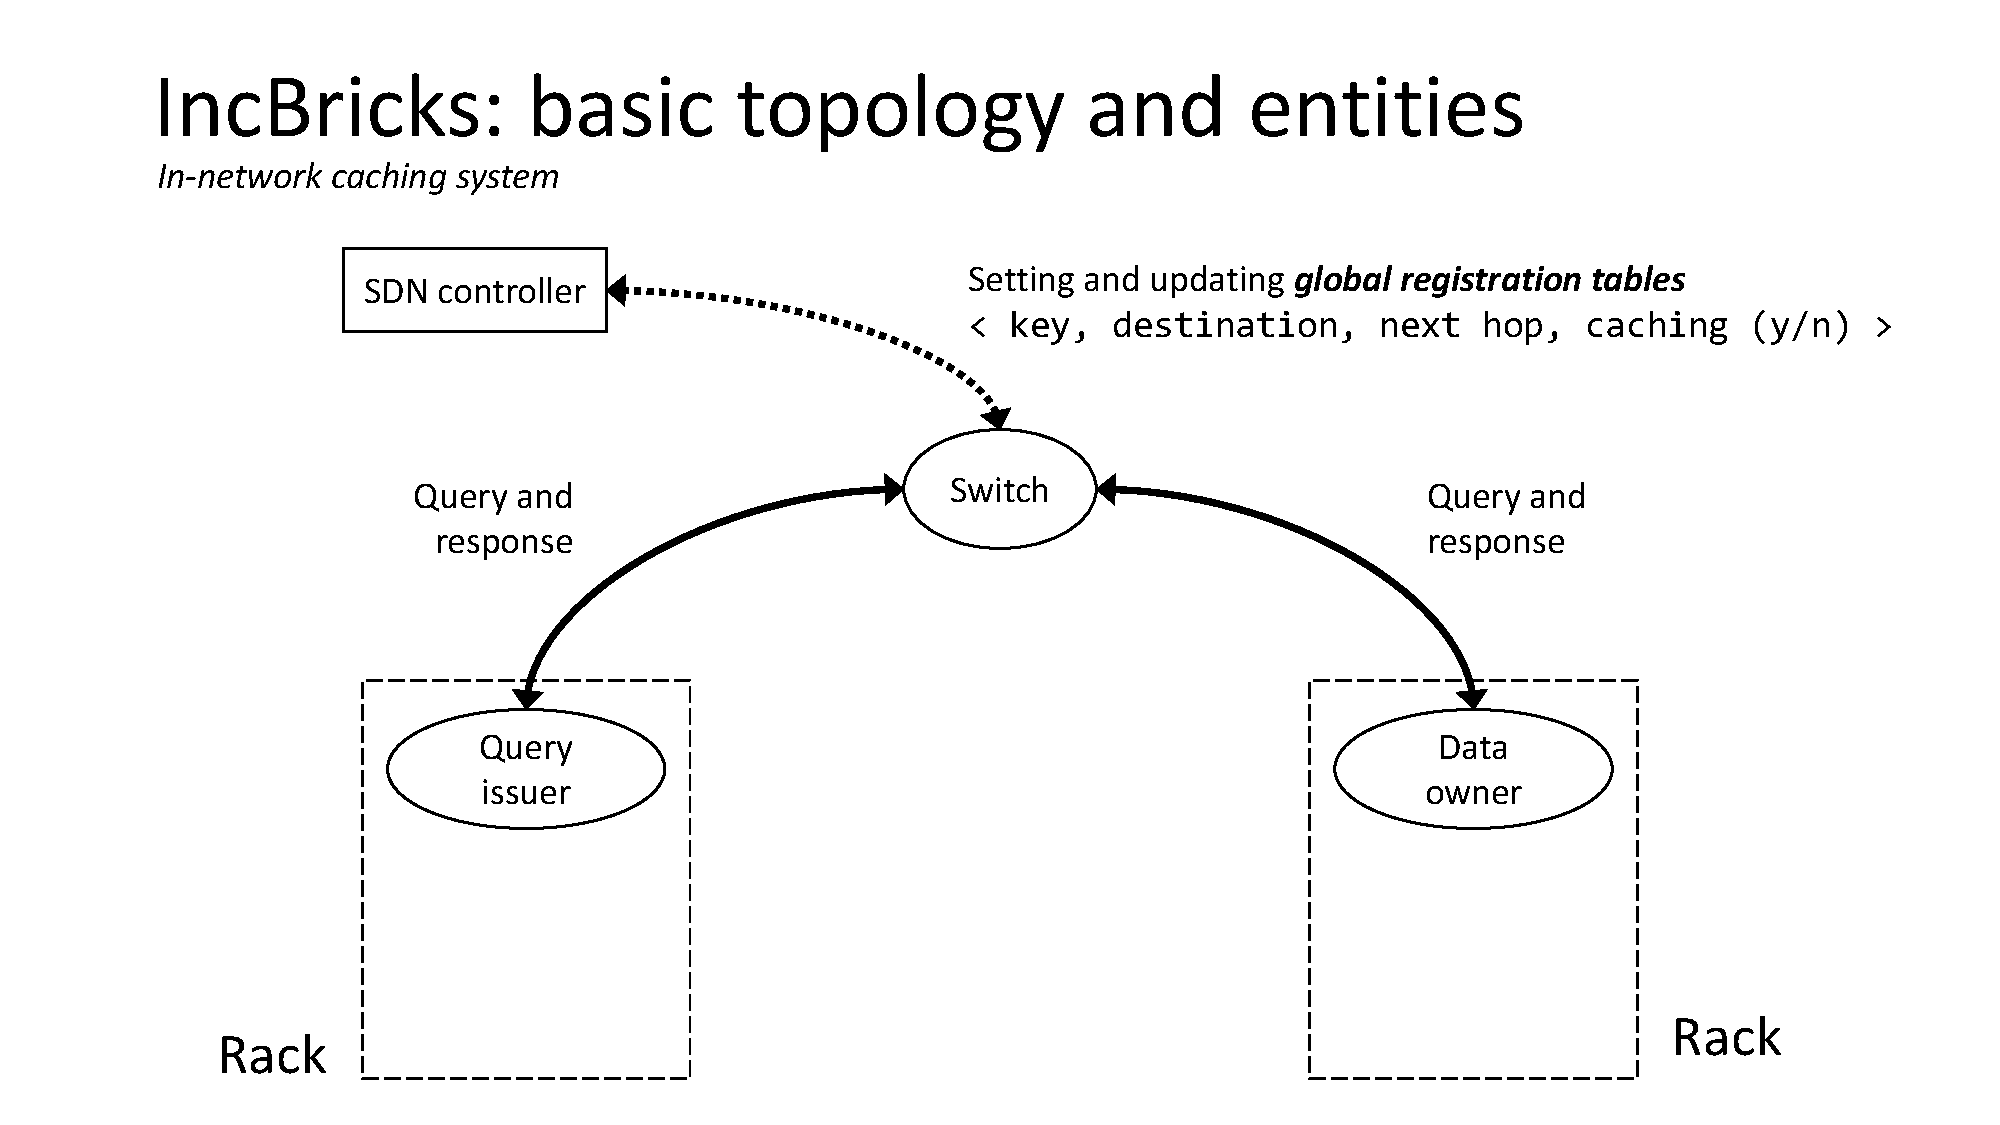
\includegraphics[page=1, clip, trim=3.6cm 0.7cm 2.5cm 4.15cm, width=0.9\textwidth]{figures/analysis/inp/solutions.pdf}
}

\newsavebox\incbricksextended \savebox\incbricksextended{
    % trim = left, bottom, right, top
    \includegraphics[page=2, clip, trim=3.6cm 0.7cm 2.5cm 4.15cm, width=0.9\textwidth]{figures/analysis/inp/solutions.pdf}
}

\newsavebox\incbrickscommunication \savebox\incbrickscommunication{
    % trim = left, bottom, right, top
    \includegraphics[page=3, clip, trim=3.6cm 0.7cm 2.5cm 4.15cm, width=0.9\textwidth]{figures/analysis/inp/solutions.pdf}
}

\newsavebox\incbrickssd \savebox\incbrickssd{
    % trim = left, bottom, right, top
    \includegraphics[page=4, clip, trim=4.1cm 0.1cm 4.3cm 0.1cm, width=0.95\textwidth]{figures/analysis/inp/solutions.pdf}
}

% SHArP
\newsavebox\sharpbasic \savebox\sharpbasic{
    % trim = left, bottom, right, top
    \includegraphics[page=13, clip, trim=3.6cm 1.3cm 3.6cm 4.8cm, width=0.9\textwidth]{figures/analysis/inp/solutions.pdf}
}

\newsavebox\sharpextended \savebox\sharpextended{
    % trim = left, bottom, right, top
    \includegraphics[page=14, clip, trim=2.4cm 0.7cm 1.8cm 3.6cm, width=0.9\textwidth]{figures/analysis/inp/solutions.pdf}
}

\newsavebox\sharpcommunication \savebox\sharpcommunication{
    % trim = left, bottom, right, top
    \includegraphics[page=15, clip, trim=3.3cm 0.9cm 1.6cm 4.6cm, width=0.9\textwidth]{figures/analysis/inp/solutions.pdf}
}

\newsavebox\sharpsd \savebox\sharpsd{
    % trim = left, bottom, right, top
    \includegraphics[page=16, clip, trim=3.6cm 0.3cm 3.7cm 0.2cm, width=0.95\textwidth]{figures/analysis/inp/solutions.pdf}
}

% Resource models and their variations
\newsavebox\vcfigure \savebox\vcfigure{
    % trim = left, bottom, right, top
    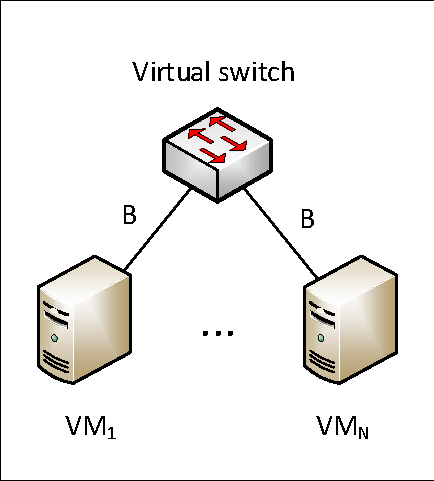
\includegraphics[page=1, clip, trim=0.5cm 0.6cm 0.5cm 1cm, width=0.34\textwidth]{figures/analysis/models/solutions.pdf}
}

\newsavebox\vocfigure \savebox\vocfigure{
        % trim = left, bottom, right, top
        \includegraphics[page=2, clip, trim=0.5cm 0.6cm 0.5cm 0.7cm, width=0.75\textwidth]{figures/analysis/models/solutions.pdf}
}

\newsavebox\tagfigure \savebox\tagfigure{
    % trim = left, bottom, right, top
    \includegraphics[page=3, clip, trim=0.5cm 0.5cm 0.5cm 0.5cm, width=0.7\textwidth]{figures/analysis/models/solutions.pdf}
}
\newsavebox\vcmodfigure \savebox\vcmodfigure{
    % trim = left, bottom, right, top
    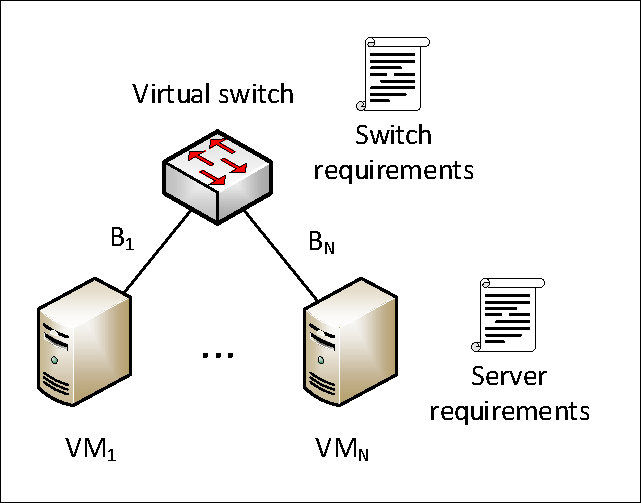
\includegraphics[page=1, clip, trim=0.6cm 0.6cm 0.6cm 0.6cm, width=0.45\textwidth]{figures/design/model/variants.pdf}
}

\newsavebox\vocmodfigure \savebox\vocmodfigure{
    % trim = left, bottom, right, top
    \includegraphics[page=2, clip, trim=0.6cm 0.6cm 0.6cm 0.6cm, width=0.95\textwidth]{figures/design/model/variants.pdf}
}

\newsavebox\tagmodfigure \savebox\tagmodfigure{
    % trim = left, bottom, right, top
    \includegraphics[page=3, clip, trim=0.6cm 0.6cm 0.6cm 0.6cm, width=0.95\textwidth]{figures/design/model/variants.pdf}
}

% Resource managers
\newsavebox\ontacklingfirststep \savebox\ontacklingfirststep{
    % trim = left, bottom, right, top
    \includegraphics[page=7, clip, trim=6.7cm 0.65cm 6.7cm 6.6cm, width=0.9\textwidth]{figures/analysis/rm/discussion.pdf}
}

\newsavebox\ontacklingsecondstep \savebox\ontacklingsecondstep{
    % trim = left, bottom, right, top
    \includegraphics[page=8, clip, trim=6.3cm 1.1cm 6.25cm 6.6cm, width=0.9\textwidth]{figures/analysis/rm/discussion.pdf}
}

\newsavebox\ontacklinginefficientswitchplacement \savebox\ontacklinginefficientswitchplacement{
    % trim = left, bottom, right, top
    \includegraphics[page=12, clip, trim=0.1cm 1.2cm 0.1cm 1cm, width=0.95\textwidth]{figures/analysis/rm/discussion.pdf}
}

% System design
\newsavebox\compositestological \savebox\compositestological{
    % trim = left, bottom, right, top
    \includegraphics[page=4, clip, trim=4.3cm 0.2cm 4.3cm 7.65cm, width=0.95\textwidth]{figures/design/model/presentation.pdf}
}

\newsavebox\logicaltophysical \savebox\logicaltophysical{
    % trim = left, bottom, right, top
    \includegraphics[page=5, clip, trim=11.2cm 3.7cm 0.6cm 3.6cm, width=0.9\textwidth]{figures/design/model/presentation.pdf}
}

\newsavebox\compositestophysical \savebox\compositestophysical{
    % trim = left, bottom, right, top
    \includegraphics[page=6, clip, trim=0.35cm 2.1cm 0.35cm 5cm, width=0.95\textwidth]{figures/design/model/presentation.pdf}
}

\newsavebox\passivemapping \savebox\passivemapping{
    % trim = left, bottom, right, top
    \includegraphics[page=7, clip, trim=3.75cm 1.05cm 3.05cm 3.8cm, width=0.95\textwidth]{figures/design/model/presentation.pdf}
}

\newsavebox\activemapping \savebox\activemapping{
    % trim = left, bottom, right, top
    \includegraphics[page=8, clip, trim=2.1cm 1.95cm 1.8cm 4.1cm, width=0.95\textwidth]{figures/design/model/presentation.pdf}
}

% Cover
\begin{titlepage}
    \begin{center}
        \vspace*{7cm}
 
        \Huge
        \textbf{Data center resource management for in-network processing}
 
        \vspace{1cm}
        
        \huge
        Marco Micera
 
        \vfill
 
        \LARGE
        \textit{Politecnico di Torino, TU Darmstadt}
    \end{center}
\end{titlepage}
% \afterpage{\blankpage}

% Table of contents
\tableofcontents
\glsresetall

% Chapters
\chapter{Introduction} \label{introduction}
This Master's thesis has been written at the Technische Universit{\"a}t Darmstadt, Germany, during a six-month Erasmus+ exchange and under the supervision of Prof. Patrick Eugster \footnote[2]{\label{tuda} Distributed Systems Programming Group, Technische Universit{\"a}t Darmstadt}, M.Sc. Marcel Bl{\"o}cher \footref{tuda} and Prof. Fulvio Risso \footnote[3]{\label{polito} Computer Networks Group, Politecnico di Torino}.

\section{Abstract}
Data centers distributed systems can nowadays make use of in-network computation to improve several factors: \textsc{Daiet} \cite{daiet} inventors claim to achieve a 86.9\%-89.3\% traffic reduction by performing data aggregation entirely in the network data plane.
Other solutions like \textsc{NetChain} \cite{netchain} and \textsc{IncBricks} \cite{incbricks} let programmable switches store data and process queries in order to cut end-to-end latency.
It is now even possible to provide guarantees to applications with specific requirements: for instance, \textsc{CloudMirror} \cite{cloudmirror} enables applications to reserve a minimum bandwidth.\par
For the time being, it seems that there is still no valid resource allocation algorithm that takes into account the presence of a network having a data plane that is (in part o completely) capable of basic \gls{inp} operations.
The objective of this thesis is to model and evaluate an \gls{api} through which applications can ask for resources in a data center exploiting \gls{inp} capabilities while providing guarantees (e.g., bandwidth).

\section{Problem statement}
Using \gls{inp} to keep scaling data centers' performance seems a promising idea: Daiet \cite{daiet} inventors claim to achieve a 86.9\%-89.3\% traffic reduction, hence reducing servers' workload; NetChain \cite{netchain} can process queries entirely in the network data plane, eliminating the query processing at servers and cutting the end-to-end latency to as little as half of an RTT.\\
Current data center \glspl{rm} (e.g., Apache YARN \cite{yarn}, Google Omega \cite{omega}) are not completely network-unaware: for instance, some of them are capable of satisfying affinity rules. CloudMirror \cite{cloudmirror} even provides bandwidth guarantees to tenant applications. Still, current \glspl{rm} do not consider \gls{inp} resources.\\
As a consequence, tenant applications cannot request \gls{inp} services while asking for server resources.

\subsection{Modeling \texorpdfstring{\glsentryshort{inp}}{INP} resources}
This Master's thesis goal consists in investigating how to model \gls{inp} resources and how to integrate them in RMs.\par
In order to offer \gls{inp} services to a tenant application, the latter should be capable of asking for \gls{inp} resources through an \gls{api}. To do that, \gls{inp} resources must be modeled not only to support currently existing \gls{inp} solutions such as \cite{daiet} \cite{netchain} \cite{incbricks} \cite{sharp}, but also to support future ones. It might be convenient to derive a single model to describe both server and \gls{inp} resources.\par
Classic tenant application requests can often be modeled as a key-value data structure. CloudMirror \cite{cloudmirror} requires a \gls{tag} as an input, which is a directed graph where each vertex represents an application component and links' weights represent the minimum requested bandwidth. One possible model could be based on a \gls{tag}, describing network resources and/or \gls{inp} services as vertexes or links. Tenants applications could either use the same model used within the data center or a simplified one, adding another level of abstraction.\par
Finally, a network-aware placement algorithm in the Resource Manager should then be able to allocate the requested resources accordingly.
\chapter{Background} \label{background}
The aim of this chapter is to introduce currently existing technologies exploited in data centers nowadays.
This chapter starts with a general description of how resource are managed in a data center \autoref{rm_background} (e.g., Virtual Machines) and ends with a brief introduction to network techniques and concepts which are strictly related to Resource Managers.

\section{Resource management in data centers} \label{rm_background}
In a data center, resources of any kind are being virtualized in order to achieve higher flexibility, portability and availability.
Usually both compute and storage resources are virtualized by means of \glspl{vm} and/or containers.
Flexibility and portability are both automatically achieved thanks to this resource virtualization, resulting in software that can be deployed dynamically, run by multiple platforms and even live migrated; availability is usually simply achieved by not co-locating \glspl{vm} in a single server or rack.

Furthermore, a Resource Manager's aim is to manage all resources in a cluster and to schedule applications (sometimes referred as \textit{jobs}) assigning the corresponding \glspl{vm}/containers to the \textit{best} subset of servers.

Today there are multiple Resource Managers that are using different approaches to solve different design issues.
This section examines these existing \glspl{rm}, trying to categorize them based on how they face different scheduling problems.

\subsection{Glossary}
\input{chapters/background/rm/glossary/intro.tex}

\subsubsection{Physical architecture}
\input{chapters/background/rm/glossary/architecture.tex}

\subsubsection{Resources}
\input{chapters/background/rm/glossary/resources.tex}

\subsection{Scheduling architectures} \label{rm_architectures}
\paragraph{Monolithic}
Probably the most simple scheduler architecture out there: a monolithic scheduler consists in a single instance scheduler applying the same scheduling algorithm for every incoming job (so there is no concurrency between resource requesters).
A centralized scheduling logic can support a more refined job placement.
On the other hand, the absence of parallelism causes an higher latency with respect to other architectures.
Although the single instance could distinguish among different job types hence treating those differently, its maintenance is not trivial, due to its single instance (and code base) nature.

\paragraph{Two-level}
This architecture requires computer clusters to be dynamically partitioned in sub-clusters, each having a dedicated scheduler.
A centralized resource allocator determines which and how many resources should made be available to each scheduler: this is done by sending \textit{offers} to schedulers (\textit{pessimistic concurrency}).
Obviously conflicts can be avoided by not offering the same resource to multiple schedulers at the time.
The same entity is in charge of dynamically divide clusters into sub-clusters: this is done to avoid resource fragmentation.

\paragraph{Shared-state}
Schedulers are not mapped to sub-clusters anymore.
Multiple schedulers have access to the entire cluster and there is no centralized resource allocator assigning resources to schedulers.
In this architecture, schedulers will try to acquire resources (\textit{optimistic concurrency}), having not only the possibility of choosing between all the resources in the cluster, but also to ask for those who have been already acquired by another scheduler.
In order to achieve this, a centralized data structure called \textit{cell state} maintains all the resource allocation information in the cluster, providing in fact a \textit{shared-state} of it.
Schedulers will try to acquire resources by atomically modifying this cell state, that will actually be modified only if the request does not cause any conflict.
Each scheduler makes its own resource-allocation decision on a private copy of the cell state, which is updated every time the scheduler tries to acquire some resource, no matter what the outcome of the attempt is.

\subsection{Taxonomy} \label{rm_taxonomy}
This section tries to underline the different scheduling design issues that \glspl{rm} must face by building a simple short taxonomy, following the guidelines provided by Google in their Omega \cite{omega} paper.

\paragraph{Scheduling work partitioning}
The workload can be distributed across schedulers basically in three different ways:
\begin{mylist}
    \item workload-type unaware load balancing,
    \item workload partitioning to specialized clusters and,
    \item a combination of the two
\end{mylist}.

\paragraph{Interference}
Schedulers can concurrently ask for the same resources.
In the pessimistic approach different resources are offered to different schedulers, making it impossible for them to compete for the same resource: this of course represents a lack of parallelism, since resource offers are made by a logically centralized entity.
The optimistic approach instead lets every scheduler claim the desired resources and just conflicting requests are denied, which of course introduces an overhead.
Of course, there could be no interference in case there is only one scheduler.

\paragraph{Choice of resources}
Schedulers can pick amongst
\begin{mylist}
    \item all cluster resources or 
    \item a subset of those
\end{mylist}.
When resources are divided into disjoint sets there will be no concurrency by definition.
Making all resources available to all scheduler will make it easier for schedulers to place jobs with particularly stringent needs, and it is also useful when the scheduling decision must be taken based on overall state (e.g., the amount of free resources in the cluster).

\paragraph{Preemption}
Schedulers can be either allowed to preempt other schedulers' job assignments or not.
Allowing preemption brings a greater flexibility at the cost of interrupting an already-running job.

\paragraph{Allocation granularity}
Considering that jobs contain multiple tasks that can be scheduled on different resources, schedulers can either
\begin{mylist}
    \item incrementally schedule tasks as soon as new resources become free or
    \item schedule a job only when all tasks can be scheduled on the spot
\end{mylist}.
Not all job types can exploit the incremental resource acquisition.
This technique can also bring the system to a deadlock if there is no back-off mechanism that releases resources once a job cannot acquire all resources in a reasonable amount of time.

\section{\texorpdfstring{\glsentryfull{inp}}{In-Network Processing (INP)}} \label{inp_background}
\subsection{A definition}
% Not general enough: this is just data center INP

% Within this project, \gls{inp} refers to the technique that exploits network switches to modify and/or store data packets, without involving any kind of higher-layer devices.
% Therefore, approaches that make use of middle-boxes do not fall within our definition of INP.
% This is why \gls{inp} is different from \textit{active networking} and \gls{nfv}.

\subsection{Examples}

\section{\texorpdfstring{\glsentryfull{nfv}}{Network Function Virtualization (NFV)}} \label{nfv_background}
\glsreset{sdn}
\glsreset{nfv}
\glsreset{inp}
\Cref{background} introduced how resources can be managed in a data center (\autoref{rm_background}) and different network techniques such as \gls{sdn} (\autoref{sdn_background}), \gls{nfv} (\autoref{nfv_background}) and \gls{inp} (\autoref{inp_background}).
This chapter aims to dig into the details of these systems and to extract common patterns between similar \gls{inp} solutions to then derive a model capable of fully describing \gls{inp} resources.

\subsection{Examples}
\chapter{Analysis} \label{analysis}
\Cref{background} introduced how resources can be managed in a data center (\autoref{rm_background}) and different network techniques such as \gls{inp} (\autoref{inp_background}) and \gls{nfv} (\autoref{nfv_background}).
This chapter's aim is to dig into the details of these systems and to extract common patterns between similar \gls{inp} solutions in order to be able to derive a model capable of fully describing \gls{inp} resources.

\section{\texorpdfstring{\glsentryfullpl{rmf}}{Resource Management Frameworks (RMFs)} analysis}
After having described the basics behind resource management in \autoref{rm_background}, it is time now to dig into the details of existing \glspl{rm} currently out there and to categorize them following the taxonomy introduced in \autoref{rm_taxonomy}.

\subsection{Borg \texorpdfstring{\cite{borg}}{}}
Borg \cite{borg} is the first container-management system developed by Google.
Jobs are divided in two groups depending on their workload type (long-running and batch) and they were initially scheduled by a logically centralized controller called \textit{Borgmaster}.
After Google developed the shared-state Omega \cite{omega} scheduler (analyzed in \autoref{omega}), Borg \cite{borg} adopted the shared-state architecture as well, hence being no more a monolithic solution.

\subsubsection{Scheduling}
Each cell has its own logically centralized controller called \textit{Borgmaster}, which is essentially split in two parts:
\begin{mylist}
    \item the scheduling part, consisting in one or more schedulers differentiated by the workload type they handle and
    \item a management unit in charge of handling client \glspl{rpc} and communicating with all other Borg \cite{borg} agents
\end{mylist}.
Schedulers mainly work on tasks rather than jobs.
Tasks are scanned in a round-robin fashion and their priority is also taken into account.
Schedulers must first find all available machines for the task to be scheduled (also considering those currently acquired by a task with lower priority) and then find the best machine amongst them all.
This second part is done by taking into consideration not only user-specified preferences, but also data center global goals like minimizing of preempted tasks and allocating tasks on machines which already have the needed packages installed in order to reduce the installation time, which usually takes about 80\% of the total start-up latency.

\subsubsection{Details}
\paragraph{Jobs}
Jobs in Borg \cite{borg} are split into multiple tasks which run within a single cell: tasks belonging to one job cannot be spread amongst multiple cells in the same cluster.
In fact, Borg \cite{borg} only operates on cells.
Each job has some properties such as a name, an owner, and most importantly, constraints about \textit{machines} (e.g., processor architecture, etc.) which will determine where its tasks will be scheduled.
Tasks instead have \textit{resource} requirements (e.g., CPU cores, RAM, etc.) expressed in terms of \textit{quotas} (an array of resource quantities).
Task properties can be modified at run-time by the job owner: this is done by pushing a new job configuration file to Borg \cite{borg} and ordering the scheduler to update the involved tasks via a non-atomic transaction.
Most of the workload in Borg \cite{borg} run in containers rather than \glspl{vm} to avoid the virtualization overhead.
\paragraph{Fairness}
Jobs have a priority expressed as an integer.
Workload types are even more differentiated with the definition of non-overlapping priority bands, one for a different kind of workload.
Borg \cite{borg} schedulers are preemptive, and in order to contain the negative effects of preemption cascades the system does not allow internal preemption for certain priority bands.
\paragraph{Resource reclamation}
Tasks do not fully use their resources for their entire lifespan.
This is why the \textit{Borgmaster} estimates every few seconds what is the actual amount of resources that each task needs and reclaims the unused resources to make them available for other tasks.
This is done by periodically contacting Borg \cite{borg} agents running on each cluster machine, requesting for fine-grained resource consumption information.
The initial estimated amount of resources actually needed by a task corresponds with its maximum limit, and it then slows according to the actual consumption.
If the actual resource usage exceeds the estimation, than the latter is rapidly increased.
This technique justifies why Borg \cite{borg} inventors have noticed that dedicating clusters for different workload types is inconvenient.
They showed how segregating long-running and batch jobs in different specialized clusters requires 20\% to 30\% more machines than having clusters who run both type of jobs using resource reclamation.

% \subsubsection{Characteristics}
    % Architecture:
    % Scheduling work partitioning:
    % Interference:
    % Choice of resources:
    % Preemption:
    % Allocation granularity:
\newpage

\subsection{Omega \texorpdfstring{\cite{omega}}{}} \label{omega}
Omega \cite{omega} is a parallel, lock-free and optimistic cluster scheduler by Google.
As said in \cite{borgomegakubernetes}, it was born after Borg \cite{borg} with the aim of improving its software engineering.
There is no central resource allocator: all of the resource-allocation decisions take place in the schedulers.
Multiple schedulers were first introduced in Omega \cite{omega} and then in Borg \cite{borg}, making the latter scheduler no more monolithic.

\subsubsection{Scheduling}
This solution makes use of a data structure called \textit{cell state} containing information about all the resource allocation in the cluster.
Each cell has a shared copy of this data structure, and each scheduler is given a private, local, frequently-updated copy of cell state that it uses for making scheduling decisions.
According to the optimistic concurrency technique, once a scheduler makes a placement decision, it updates the shared copy of cell state with a transaction.
Whether or not the transaction succeeds, a scheduler re-syncs its local copy of cell state afterwards and, if necessary, re-runs its scheduling algorithm and tries again.
Omega \cite{omega} supports specialized schedulers: authors have showed the advantages of a MapReduce \cite{mapreduce} specialized scheduler in \cite{omega}.

\subsubsection{Conclusions}
Since schedulers do not have access to all cluster resources, Mesos \cite{mesos} cannot support preemption across different sub-clusters and it cannot apply policies that make use of the complete cluster state.

% \subsubsection{Characteristics}
    % Architecture:
    % Scheduling work partitioning:
    % Interference:
    % Choice of resources:
    % Preemption:
    % Allocation granularity:
\newpage

\subsection{\texorpdfstring{\glsdesc{yarn_full}}{}}
\glsdesc{yarn_full} (for the sake of brevity: \glsdesc{yarn}) is the Resource Manager of \glsdesc{hadoop}, a framework for distributed processing across clusters.\par
\glsdesc{hadoop} was initially an open source implementation of MapReduce \cite{mapreduce}, but then the programming model has been separated from the resource management function, resulting in an application-independent \gls{rm} known as \glsdesc{yarn}.

\subsubsection{Entities}
For each tenant application there is an \textit{Application Master} whose task is to
\begin{mylist}
    \item manage the application life cycle and
    \item negotiate the resources that the application needs with the central \gls{rm}, making \glsdesc{yarn} a monolithic scheduler with no interference between tenant applications
\end{mylist}.
Each node then has a \textit{Node Manager} thanks to which the \gls{rm} can allocate tasks on it.
The \textit{Node Manager} must also periodically monitor resource availability and report failures.

\subsubsection{Scheduling}
Application Masters issue resource request to the \gls{rm}, containing containers properties and locality preferences.
Upon receiving a resource request, the centralized scheduler generates containers using available resources periodically advertised by the nodes themselves.
The outcome of this procedure is reported to the Application Master corresponding to the tenant application who initiated the request.
Application Masters are also informed upon inserting new nodes into the system.

\subsubsection{Details}
\paragraph{Preemption}
The \gls{rm} can also ask to Application Masters to revoke some resources in case of a shortage.
The application will then have a few choices: for instance it can yield containers that are less important or checkpoint its current status.
If an application does not collaborate with the \gls{rm} upon receiving a \textit{revoking request}, the \gls{rm} will forcibly terminate those targeted containers.
\paragraph{Failures}
The \gls{rm} represents a single point of failure for the system and its restart causes the termination of all containers in the cluster, including all their Application Masters.
Node failures are detected by the \gls{rm} using timeouts (nodes have to periodically contact the \gls{rm}).
The \gls{rm} will then inform all Application Masters who are responsible for responsible for the application life cycle.

\subsubsection{Conclusions}
Undoubtedly, \glsdesc{yarn} dedicates less attention to scalability due to its de facto monolithic scheduler: there are multiple Application Masters who just take care of the application life cycle and do not perform scheduling, which is done instead by a single \gls{rm}.\par
However, \glsdesc{yarn} authors state that the centralized \gls{rm} can assure fairness, capacity and locality thanks to the central and global view that it has on the system.
They justify this by pointing out that \glsdesc{hadoop} is an open platform which lets different independent sources share the same cluster, unlike other "\textit{closed-world}" schedulers like Google Omega \cite{omega}.

% \subsubsection{Characteristics}
    % Architecture:
    % Scheduling work partitioning:
    % Interference:
    % Choice of resources:
    % Preemption:
    % Allocation granularity:
\newpage

\subsection{Mesos \texorpdfstring{\cite{mesos}}{}}
% Mesos, on the other hand, is a widely-deployed production cluster manager which supports multi-dimensional resource requirements [GZH+11], but does not explicitly consider co-location interference.

Mesos \cite{mesos} is a two-level cluster scheduler based on \textit{resource offers}.
It has multiple schedulers since Mesos \cite{mesos} has been conceived to share clusters between different cluster computing frameworks since the beginning of its development.
By contrast, \glsdesc{yarn} was initially embedded in the first version of MapReduce \cite{mapreduce} and subsequently became independent out of the necessity to scale \glsdesc{hadoop}.

\subsubsection{Entities}
This scheduler has a logically centralized resource \textit{allocator} in charge of offering resources to different schedulers.
It is called \textit{Mesos master} and it is replicated for fault tolerance.
A scheduler with its \textit{executor} (worker) node are together called \textit{framework}.
Nodes running on cluster nodes are called \textit{Mesos slaves}.

\subsubsection{Scheduling}
Initially, every cluster node reports to the master node its own available resources.
Based on this data, the master node can then offer resources to application frameworks based on a particular policy.
The master node does not offer the same subset of resources to each scheduler.
Obviously resource conflicts can be avoided by not offering the same resource to multiple schedulers at the time.
Upon receiving resources offers, application frameworks can either reject the offer (in case it does not satisfy all framework's constraints) or tell the master which tasks need to be run on the dedicated resources.
Mesos \cite{mesos} already knows that certain types of frameworks always reject certain resource offers characterized by some factors, so frameworks can specify \textit{filters} in order for the master to automatically avoid proposing certain kind of resources.\par
The resource allocation logic can be customized, and Mesos \cite{mesos} includes an allocation module based on priority and one based one fairness.
Tasks can be preempted, however frameworks can be offered \textit{guaranteed} resources on which tasks cannot be preempted.


% \subsubsection{Characteristics}
    % Architecture:
    % Scheduling work partitioning:
    % Interference:
    % Choice of resources:
    % Preemption:
    % Allocation granularity:
\newpage

\subsection{Guarantee provisioning: CloudMirror \texorpdfstring{\cite{cloudmirror}}{}}
CloudMirror \cite{cloudmirror} allows client applications to specify bandwidth and high availability guarantees.

\subsubsection{Motivation} \label{why_tag}
Prior models are not suitable to represent interactive non-batch applications with very stringent bandwidth requirements.
Both the hose and the \gls{voc} model are inefficient as they over-allocate bandwidth.
The main reason of why this happens is that both models \textit{aggregate} bandwidth requirements between different application components into a single hose: as a consequence, the \gls{vm} scheduler does not get to know the actual bandwidth needed between application components.
At the opposite extreme there is the pipe model which, besides not exploiting statistical multiplexing, is not scalable since it requires a list of all bandwidth guarantees between pairs of \glspl{vm}.
This led CloudMirror \cite{cloudmirror} inventors to come up with a new model.

\subsubsection{Tenant Application Graph} \label{tag_description}
The \gls{tag} is a directed graph where each vertex represents an application component and links' weights represent the minimum requested bandwidth. Each vertex can have an optional \textit{size}, denoting the number of \glspl{vm} belonging to the component.

\begin{figure}[!htb]
    \centering
    \usebox{\tagfigure}
    \caption{A \gls{tag} example}
\end{figure}

There are two types of edges:
\begin{mylist}
    \item self-loop edges, that are equivalent a hose model and
    \item standard vertex-to-vertex edges
\end{mylist}.
A standard edge from $Tier 1$ to $Tier 2$ is labeled with an ordered pair of numbers $<SB_12, RB_12>$, indicating respectively the guaranteed bandwidth with which \glspl{vm} in $Tier 1$ can send traffic to \glspl{vm} in $Tier 2$ and the guaranteed bandwidth with which \glspl{vm} in $Tier 2$ can receive traffic from \glspl{vm} in $Tier 1$.

\subsubsection{Model advantages}
The edge label format $<S, R>$ allows the model to exploit statistical multiplexing, since $S$ can represent the peak of the sum of \gls{vm}-to-\gls{vm} demands instead of the (typically larger) sum of peak demands needed by the pipe model.
\textbf{\textit{TO BE CONTINUED}} ...

% An heuristic \gls{vm} placement algorithm then tries to solve this NP-hard allocation problem.

% \subsubsection{Characteristics}
    % Architecture:
    % Scheduling work partitioning:
    % Interference:
    % Choice of resources:
    % Preemption:
    % Allocation granularity:
\newpage

\subsection{Firmament \texorpdfstring{\cite{firmament}}{}}
Firmament \cite{firmament} is a centralized cluster scheduler capable of supporting multi-dimensional resource requirements (\autoref{firmament:multi-dimensions}).
The scheduler finds an embedding solution by solving a min-cost max-flow optimization problem over a graph called \textit{flow network} (\autoref{firmament:flow_network}).

\subsubsection{Flow network} \label{firmament:flow_network}
The flow network is a directed weighted graph that contains both \glslink{resource:physical}{physical} and \glspl{resource:logical}.
Similarly to any other graph-based scheduler (e.g., \cite{ontackling}), a \gls{resource:physical} is connected to a \gls{resource:logical} anytime the former can be allocated on the latter.
In order to reduce the overall amount of arcs, the flow network makes use of \textit{equivalence class aggregates} which group nodes with similar characteristics (e.g., tasks within a job, physical machines with the same micro-architectural topology, etc.).
An aggregate receives arcs from all entities belonging to it.
Physical aggregates can also receive arcs from those logical nodes that can be allocated on any of the physical entity represented by the aggregate.\par
The physical network is faithfully recreated in the graph thanks to aggregates: for instance, different machines belonging to the same rack are connected to the same \textit{rack aggregate}, all racks are connected to the cluster aggregate and so on.
The description does not either stop at the machine level, since also sockets and cores are represented in the graph.
Again, inclusion relationships are expressed in terms of arcs.
Special \textit{unscheduled aggregates} (one for each job) receive an arc from every task.\par
The embedding solution is found by running an instance of a min-cost max-flow optimization algorithm over the network flow.
If a task cannot be allocated on any of the physical machines, its flow will be directed to its corresponding unscheduled aggregate.
Arcs' costs are determined by a given scheduling policy (or "cost model"): at the time of writing, Firmament \cite{firmament} supports 9 different scheduling policies.
Intuitively, arcs connecting tasks to unscheduled aggregates will have an higher cost with respect to the ones ending in a physical entity.

\subsubsection{Multi-dimensional resource fitting} \label{firmament:multi-dimensions}
Firmament's \cite{firmament} creator Malte Schwarzkopf introduced the coordinated co-location (CoCo) cost model in his PhD dissertation - Schwarzkopf, M. (2018). \textit{Operating system support for warehouse-scale computing} (Doctoral thesis). \href{https://doi.org/10.17863/CAM.26443}{https://doi.org/10.17863/CAM.26443}.\par
This scheduling policy has an interesting feature: \textit{admission control}.
Basically a task can be allocated on a physical machine only when it satisfies all task's resource requirements (strict resource fit).
If a task cannot be allocated on any of the physical machines, it cannot be even connected to the cluster aggregate.
Given a \gls{resource:logical} in the network flow, CoCo is able to efficiently determine all subtrees in the physical topology in which it can be allocated.
This is done by storing in each physical aggregate the minimum and maximum amount of available resources across its children.
\newpage

\subsection{\texorpdfstring{\glsentryshortpl{rmf}}{RMFs} comparison}
The table below contains a quick comparison amongst \glspl{rm} previously analyzed.
In order to categorize those, the taxonomy introduced in \autoref{rm_taxonomy} has been used.

\begin{table}[h]
\begin{center}
\begin{tabular}{lll}

\multicolumn{3}{c}{\textbf{Resource Managers: quick summary}} \\ \hline
\multicolumn{1}{l|}{\textbf{Borg \cite{borg}}} 
                                   & Scheduling architecture      & Shared-state            \\ \cline{2-3} 
\multicolumn{1}{l|}{}              & Scheduling work partitioning & Specialized clusters    \\ \cline{2-3} 
\multicolumn{1}{l|}{}              & Interference                 & Optimistic approach     \\ \cline{2-3} 
\multicolumn{1}{l|}{}              & Choice of resources          & All cluster resources   \\ \cline{2-3}  
\multicolumn{1}{l|}{}              & Preemption                   & Yes                     \\ \cline{2-3} 
\multicolumn{1}{l|}{}              & Allocation granularity       &                         \\ \cline{2-3}

\multicolumn{3}{c}{} \\ \hline
\multicolumn{1}{l|}{\textbf{Omega \cite{omega}}} 
                                   & Scheduling architecture      & Shared-state            \\ \cline{2-3} 
\multicolumn{1}{l|}{}              & Scheduling work partitioning & Specialized clusters    \\ \cline{2-3} 
\multicolumn{1}{l|}{}              & Interference                 & Optimistic approach     \\ \cline{2-3} 
\multicolumn{1}{l|}{}              & Choice of resources          & All cluster resources   \\ \cline{2-3} 
\multicolumn{1}{l|}{}              & Preemption                   & Yes                     \\ \cline{2-3} 
\multicolumn{1}{l|}{}              & Allocation granularity       & Per-scheduler policy    \\ \cline{2-3} 

\multicolumn{3}{c}{} \\ \hline
\multicolumn{1}{l|}{\textbf{\glsdesc{yarn}}} 
                                   & Scheduling architecture      & Monolithic              \\ \cline{2-3} 
\multicolumn{1}{l|}{}              & Scheduling work partitioning & ---                     \\ \cline{2-3} 
\multicolumn{1}{l|}{}              & Interference                 & No interference         \\ \cline{2-3} 
\multicolumn{1}{l|}{}              & Choice of resources          & All cluster resources   \\ \cline{2-3} 
\multicolumn{1}{l|}{}              & Preemption                   & Yes                     \\ \cline{2-3} 
\multicolumn{1}{l|}{}              & Allocation granularity       &                         \\ \cline{2-3}

\multicolumn{3}{c}{} \\ \hline
\multicolumn{1}{l|}{\textbf{Mesos \cite{mesos}}} 
                                   & Scheduling architecture      & Two-level               \\ \cline{2-3} 
\multicolumn{1}{l|}{}              & Scheduling work partitioning &                         \\ \cline{2-3} 
\multicolumn{1}{l|}{}              & Interference                 & Pessimistic approach    \\ \cline{2-3} 
\multicolumn{1}{l|}{}              & Choice of resources          & Subset of resources     \\ \cline{2-3} 
\multicolumn{1}{l|}{}              & Preemption                   & Yes                     \\ \cline{2-3} 
\multicolumn{1}{l|}{}              & Allocation granularity       & All-or-nothing                    

\end{tabular}
\end{center}
\caption{Resource Managers comparison table using the taxonomy introduced in \autoref{rm_taxonomy}}
\label{rm-comparison}
\end{table}
\newpage

\section{\texorpdfstring{\glsentryshort{inp}}{INP} solutions}
State-of-the-art \gls{inp} solutions will be discussed in this section with the aim of deriving a model capable of fully describing \gls{inp} resources.
To that end, it is necessary to dig into the details and to recognize common patterns between them.

\subsection{In-network aggregation: Daiet \texorpdfstring{\cite{daiet}}{}}
Daiet \cite{daiet} is a system that performs in-network data aggregation for partition/aggregate data center applications (big data analysis such as MapReduce \cite{mapreduce}, machine learning, graph processing and stream processing).
Instead of letting worker servers entirely perform computation on the data and then communicate with each other to update shared state or finalize the computation, the system let network devices perform data aggregation in order to achieve traffic reduction, thus reducing the processing load at the destination.\par
The inventors have proven that in-network data aggregation can reduce the network traffic significantly for machine learning algorithms (e.g., TensorFlow \cite{tensorflow}) and for graph analytics algorithms (e.g., GPS \cite{gps}), hence justifying the usefulness of this system. The system has been designed for P4 \cite{p4} and programmable ASICs, and it can be used on any other \gls{sdn} platform.

\subsubsection{Details}
\paragraph{Controller}
When executing a MapReduce program, the job allocator informs the network controller of the job allocation to the workers.
Then, the network controller pushes a set of rules to network devices in order to
\begin{mylist}
    \item establish one aggregation tree for each reducer and
    \item perform per-tree aggregation
\end{mylist}.
An aggregation tree is a spanning tree from all the mappers to the reducer.

\begin{figure}[!htb]
    \centering
    \usebox{\daietbasic}
    \caption{Daiet's \texorpdfstring{\cite{daiet}}{} basic topology and entities}
\end{figure}

\paragraph{Packets}
Since every reducer has its own aggregation tree associated with it, network devices should know how to correctly forward traffic according to the corresponding tree: to achieve this, a special \textit{tree ID} (that could coincide with the \textit{reducer ID}) packet field allows network devices to distinguish different packets belonging to different aggregation trees.

\begin{figure}[!htb]
    \centering
    \usebox{\daietextended}
    \caption{Daiet's \texorpdfstring{\cite{daiet}}{} extended topology}
\end{figure}

Obviously, they must also know the output port towards the next network device in the tree and the aggregation function to be performed on the data.

\begin{figure}[!htb]
    \centering
    \usebox{\daietcommunication}
    \caption{Daiet's \texorpdfstring{\cite{daiet}}{} logical communication pattern}
\end{figure}

Packets are sent via UDP (therefore communication is not reliable) with a small preamble that specifies
\begin{mylist}
    \item the number of key-value pairs contained in the packet and
    \item the \textit{tree ID} whose packet belongs to
\end{mylist}.
They payload is not serialized to achieve a faster computation by network devices.

\subsubsection{Algorithm} \label{daiet_algorithm}
To store the key-value map, network devices use two hash tables for each tree: one for the keys and one for the values.
Upon a collision, the algorithm checks whether the key is matching or just the hash is.
In the former case, data aggregation is performed.
In the latter case, the conflicting pair will end up in a \textit{spillover bucket} that will be flushed to the next node as soon as it becomes full: this is done since this data is more likely to be aggregated by the next network device if it has spare memory.

\begin{figure}[!htb]
    \centering
    \usebox{\daietsd}
    \caption{Messages exchanged during a Daiet \texorpdfstring{\cite{daiet}}{} instance execution}
\end{figure}

A network device will also flush its data as soon as all its children (according to the aggregation tree) have sent their data: this is made possible by forcing network devices to send a special \textit{END} packet after transmitting all key-value pairs to their successor.\par
Used indexes are stored in a \textit{index stack} to avoid scanning the whole hash table when flushing.

\subsubsection{Implementation} \label{daiet_implementation} \label{p4_drawbacks}
The network data plane has been programmed using P4 \cite{p4}, which brings two main drawbacks:
\begin{mylist}
    \item a match-action table cannot be applied more than once for the same packet, forcing the programmer to perform loop unrolling in case of multiple headers in the same packet that need to be modified by the same rule table and
    \item keys must have a fixed size, causing a big waste of memory in applications where keys have variable-lengths (e.g., strings)
\end{mylist}.
The second drawback will also cause arrays to have fewer but bigger cells, thus increasing the probability of collisions.
If these collisions involve pairs having different keys (\cref{daiet_algorithm}), data will not be aggregated, causing traffic to increase.

\subsubsection{Minimum system requirements}
For each aggregation tree (i.e., for each reducer), network devices must form a tree whose root is connected to the reducer and whose leaves are connected to mappers.
Each mapper has to be connected to exactly one network device of the lowest level.
Network devices must
\begin{mylist}
    \item store two arrays (one for the keys and one for the values) and
    \item be able to hash keys
\end{mylist}.
The solution requires that the system has a centralized \gls{sdn} controller connected to all switches.
The \gls{sdn} controller must push flow rules to all switches belonging to at least one tree.

\subsubsection{Conclusions}
Besides all the drawbacks brought by P4 \cite{p4} listed in \cref{daiet_implementation}, inventors claim to achieve a 86.9\%-89.3\% traffic reduction, causing the execution time at the reducer to drop by 83.6\% on average.
\newpage

\subsection{Coordination services: NetChain \texorpdfstring{\cite{netchain}}{}}
NetChain \cite{netchain} is an in-network solution for coordination services, such as distributed locking, barriers, etc.
All these services are realized on top of a strongly-consistent and fault-tolerant key-value store, which is entirely implemented in the network data plane.
The network device in charge of storing the distributed store is a programmable switch: this brings an obvious limitation in terms of storage size, that makes NetChain \cite{netchain} an acceptable solution only when a small amount of critical data must be stored in the network data plane, e.g., coordination services.\par
NetChain \cite{netchain} can process queries entirely in the network data plane, causing the end-to-end latency to drop from multiple RTTs to as little as half of one RTT since servers are not involved in query processing anymore.

\subsubsection{Details}
\paragraph{Packets}
Custom UDP packets are used for queries, containing fields like \textit{operation}, \textit{key} and \textit{value}.
Read and write queries only involve the network data plane, while insert and delete queries involve the network controller to set up entries in switch tables and to perform garbage collection, respectively.

\begin{figure}[!htb]
    \centering
    \usebox{\netchainbasic}
    \caption{NetChain's \texorpdfstring{\cite{netchain}}{} basic topology and entities}
\end{figure}

This is acceptable since coordination services usually perform read and write queries on already-existing objects, e.g., locks.
Each switch has its own IP address, and packet headers contain the list of addresses of switches to be traversed, allowing those to properly forward packets to the their successors (from head to tail for write queries and the opposite for read queries).
\begin{figure}[!htb]
    \centering
    \usebox{\netchainsd}
    \caption{Messages exchanged during a NetChain \texorpdfstring{\cite{netchain}}{} instance execution}
\end{figure}
This list of IP addresses is inserted by the client (a NetChain \cite{netchain} agent).

\paragraph{Consistency}
A variant of Chain Replication \cite{chainreplication} is used in the data plane to handle read and write queries and to ensure strong consistency, while switches reconfiguration is handled by the network control plane.
The main difference with the standard Chain Replication \cite{chainreplication} protocol is that objects are stored on programmable switches instead of servers.
Switches are logically connected together in order to form an oriented chain.

\begin{figure}[!htb]
    \centering
    \usebox{\netchainextended}
    \caption{NetChain's \texorpdfstring{\cite{netchain}}{} extended topology}
\end{figure}

Read queries are processed by the \textit{tail} switch while write queries are sent to the \textit{head} switch, which will forward the updated state to the rest of the chain.

\begin{figure}[!htb]
    \centering
    \usebox{\netchaincommunication}
    \caption{NetChain's \texorpdfstring{\cite{netchain}}{} logical communication pattern}
\end{figure}

The key-value store is partitioned amongst \textit{virtual nodes} using consistent hashing, mapping keys to a hash ring.
Each ring segment is stored by $f + 1$ virtual nodes allocated on different physical switches, hence tolerating faults involving up to $f$ switches.

\subsubsection{Implementation}
The network data plane has been programmed in P4 \cite{p4} while the controller has been coded in Python, it runs on a server and communicates with switches through the standard Python RPC library.
Switches agents are Python processes who run in the switch OS. Some P4 \cite{p4} drawbacks were already discussed in \cref{p4_drawbacks}.\par
The out-of-order UDP delivery problem is resolved by adding sequence numbers to write queries, hence serializing those operations, while the loss of packets is coped by \textit{client-side retries} based on timeouts.

\subsubsection{Minimum system requirements}
Network devices must form a chain of length $f + 1$ in order to tolerate $f$ failures. The client must include the list of IP addresses of all the $f + 1$ switches to be traversed in each query packet header (from head to tail for write queries and the opposite
for read queries; storing the entire backward list for read queries is only necessary in case of tail failures).\par
Network devices must dedicate some local storage to NetChain \cite{netchain}: more specifically, they need to store a
\begin{mylist}
    \item register array to store values and a
    \item match-action table to store the keys' location in the register array and the corresponding action to be performed
\end{mylist}.
The solution requires that the system has a centralized \gls{sdn} controller connected to all switches.
The \gls{sdn} controller must handle switches reconfigurations.

\subsubsection{Conclusions}
NetChain \cite{netchain} inventors state that the on-chip memory of programmable switches in enough for coordination services.
Assuming a $\SI{10}{\mega\byte}$ partition allocated on each NetChain \cite{netchain} switch, a data center with 100 switches can provide a $(\SI{10}{\mega\byte} \cdot 100) / 3 = \SI{333}{\mega\byte}$ storage with a replication factor of three: that would be enough for the average number of files (22k, from 0 to 1 byte) managed by a typical Chubby \cite{chubby} lock service instance, as cited by Google in their corresponding paper.
Likewise, inventors claim that switches total memory is enough for a distributed locking system: assuming $\SI{30}{\byte}$ locks, the previously-mentioned example would be capable of storing $\SI{333}{\mega\byte} / \SI{30}{\byte} = 10M$ concurrent locks.
\newpage

\subsection{In-network caching fabric: IncBricks \texorpdfstring{\cite{incbricks}}{}}
IncBricks \cite{incbricks} is a hardware-software co-designed system for in-network caching: it makes use of network accelerators attached to programmable switches whenever complicated operations should be performed on payloads.
Supporting multiple gigabytes of memory, network accelerators overcome the limited storage problem typical of programmable switches, which usually have a memory of tens of megabytes.

\subsubsection{Details}
\paragraph{Hardware}
IncBricks \cite{incbricks} is composed by two components:
\begin{mylist}
    \item IncBox, an hardware unit consisting of a network accelerator and a programmable switch, and
    \item IncCache, a software system for coherent key-value storage
\end{mylist}.
Packets arriving to an IncBox device are first managed by the switch, which forwards the packet to the network accelerator only if it is labeled as an in-network cache one.

\begin{figure}[!htb]
    \centering
    \usebox{\incbricksbasic}
    \caption{IncBricks' \texorpdfstring{\cite{incbricks}}{} basic topology and entities}
\end{figure}

If there is a match, the programmable switch will check whether the packet has been already cached by the network accelerator or not, and will forward the packet to the right network accelerator attached to it in the former case.

\begin{figure}[!htb]
    \centering
    \usebox{\incbrickscommunication}
    \caption{IncBricks' \texorpdfstring{\cite{incbricks}}{} logical communication pattern}
\end{figure}

\paragraph{Logic}
The system has been designed having a multi-rooted tree topology in mind.
For each key the centralized \gls{sdn} controller comes up with a set of \textit{designated} IncBox units allowed to cache that key.
Any other IncBox unit placed between these designated units won't cache data with that specific key.

\begin{figure}[!htb]
    \centering
    \usebox{\incbrickssd}
    \caption{Messages exchanged during an IncBricks \texorpdfstring{\cite{incbricks}}{} instance execution}
\end{figure}

Then, for a given key and a given destination node, the \gls{sdn} controller establishes a unique path of designated IncBox units.
Every IncBox unit in the system will get to know
\begin{mylist}
    \item the set of immediate designated successors (according to the tree topology) for every key it is responsible of and
    \item the unique successor used for a given destination and a given key
\end{mylist}.
This data is stored in the so-called \textit{global registration table}.
Storing the former information can be useful in case of failures since it is possible to build alternative paths immediately, making the whole system more reliable.
As soon as a failure is detected, the \gls{sdn} controller updates all the involved tables.

\subsubsection{Implementation}
The storage has been implemented using a bucket spilling hash table plus a hash index table
\textbf{\textit{TO BE CONTINUED}} ...

\subsubsection{Minimum system requirements}
Communicating nodes (\glspl{vm}) represent the leaves of the tree.
Each path must include exactly one root switch.



All things considered, it seems reasonable to state that the actual required topology is a chain starting from a leaf, passing through a root node and ending on another leaf.

\begin{figure}[!htb]
    \centering
    \usebox{\incbricksextended}
    \caption{IncBricks' \texorpdfstring{\cite{incbricks}}{} extended topology}
\end{figure}

IncBox units must dedicate some local storage to realize the caching system.
The solution requires that the system has a centralized \gls{sdn} controller connected to all switches.
The \gls{sdn} controller must set configure network devices in order for them to forward IncBricks \cite{incbricks} packets accordingly.

\subsubsection{Conclusions}
\newpage

\subsection{Aggregation protocol: SHArP \texorpdfstring{\cite{sharp}}{}}
SHArP \cite{sharp} stands for \textit{Scalable Hierarchical Aggregation Protocol}, and it defines a protocol for reduction operations.
This solutions aims to accelerate \gls{hpc} applications by offloading some operations to the network. SHArP \cite{sharp} is targeted to support the two most used \glspl{api} in the \gls{hpc} area today: MPI \cite{mpi} and OpenSHMEM \cite{openshmem}.
The kind of operations that can be offloaded to the network are:
\begin{mylist}
    \item MPI \cite{mpi} barrier, reduce and allreduce,
    \item logic operands like sum, min, max, or, xor, and,
    \item integer and floating-point operations
\end{mylist}.

\subsubsection{Details}
\paragraph{Entities}
\glspl{an} are logical entities performing reduction operations.
Such a node can either execute on a network device or on a server, and it is implemented as a daemon, namely \texttt{sharpd}.

\begin{figure}[!htb]
    \centering
    \usebox{\sharpbasic}
    \caption{SHArP's \texorpdfstring{\cite{sharp}}{} basic topology and entities}
\end{figure}

All \glspl{an} must form an aggregation tree.
Multiple trees are allowed in a system.
Similarly to other in-network aggregation solutions like Daiet \cite{daiet}, data is aggregated along the aggregation tree by \glspl{an}, until it reaches a root \gls{an} that is in charge of distributing the result.

\begin{figure}[!htb]
    \centering
    \usebox{\sharpcommunication}
    \caption{SHArP's \texorpdfstring{\cite{sharp}}{} logical communication pattern}
\end{figure}

The protocol also introduces the concept of \textit{group}, consisting in a subset of physical hosts that are connected to the tree leaves: for instance, in MPI \cite{mpi} a group coincides with a \textit{communicator}.
One aggregation tree supports multiple groups.

Resources are managed by a special management entity called \gls{am}.
Faults and errors are always notified to this node, that will also take care of freeing all resources belonging to the tree in which the error occurred.
The detection of faults and errors cannot be done using timeouts since \gls{hpc} \glspl{api} do not bound the duration of aggregation operations: this is why faults must be necessarily detected by monitoring.

\paragraph{Data flow}
Eventually, an host program will need to execute a job on multiple nodes.
When the job is launched and all host processes have been created (e.g., a communicator in MPI \cite{mpi}), either the cluster resource manager (like Slurm \cite{slurm} or \glsdesc{ibm} Spectrum LSF) or an MPI \cite{mpi} launcher like \texttt{mpirun} will contact the \gls{am}, which will dedicate SHArP \cite{sharp} resources to the job and return back the list of these allocated resources.
At this point, a SHArP \cite{sharp} group has been created.
Each SHArP \cite{sharp} daemon \texttt{sharpd} running on every group member will establish a reliable connection to the dedicated leaf switch.
The \gls{am} informs the \glspl{an} about the switch resources allocated to the application, not allowing it to exceed the allocation.\par
Once connections have been established, all group members send an aggregation request message to their parent \gls{an}.
Each \gls{an} waits for all its children requests before sending the aggregated data piggybacked on another aggregation request to the parent node.
\glspl{an} temporarily maintain a data structure to track an aggregation operation's progress.\par
As soon as the tree root node receives data from all its children, it performs the final aggregation and it sends the result to a destination, that could be
\begin{mylist}
    \item one or more process belonging to one or more groups or
    \item an external process not belonging to any reduction group
\end{mylist}.
In the former case, the aggregation tree is used to redistribute the result.

\subsubsection{Implementation}
SHArP \cite{sharp} has been implemented using InfiniBand \cite{infiniband} as communication standard with \glsdesc{switchib2} devices, which provide support for data reduce operations and for barriers.
Nodes in the SHArP \cite{sharp} tree are InfiniBand \cite{infiniband} end nodes, and links are implemented using InfiniBand's \cite{infiniband} \textit{Reliable Connection}s.
When distributing a result using a multicast address, though, an unreliable delivery mechanism is used.
One \gls{an} can participate to at most 64 different aggregation trees.

\subsubsection{Minimum system requirements}
\glspl{an} (usually run by network devices) must form a tree whose leaves are connected to data producers (a \textit{communicator} in MPI \cite{mpi}).
Each data producer is connected to only one tree leaf.
The root \gls{an}, instead, is connected to the data consumer, which receives the final aggregated result.
\glspl{an} must dedicate part of their local memory to the system.

\begin{figure}[!htb]
    \centering
    \usebox{\sharpextended}
    \caption{SHArP's \texorpdfstring{\cite{sharp}}{} extended topology}
\end{figure}

The special management unit (\gls{am}) must act as a SHArP \cite{sharp} \gls{rm}, dedicating SHArP \cite{sharp} resources to those entities who request for them.

\begin{figure}[!htb]
    \centering
    \usebox{\sharpsd}
    \caption{Messages exchanged during a SHArP \texorpdfstring{\cite{sharp}}{} instance execution}
\end{figure}

\subsubsection{Conclusions}
For MPI \cite{mpi} applications SHArP \cite{sharp} brings a significant advantage in terms of latency: tests show that the latency improvement factor (latency experienced without SHArP \cite{sharp} divided by the one experienced with SHArP \cite{sharp}) is proportional to the message size.
Even in the worst case, with a message size of just \SI{8}{\mega\byte}, an MPI \cite{mpi} execution with SHArP \cite{sharp} is twice as fast as the one without using it.
\newpage

\section{Integrating \texorpdfstring{\glsentryshort{inp}}{INP} resources in \texorpdfstring{\glsentryfullpl{rm}}{Resource Managers (RMs)}}
There is currently no \gls{rm} nowadays that
\begin{mylist}
    \item handles all logical server, switch and edge resources,
    \item supports high-level requests (e.g., with the use of composites) and
    \item is capable of considering multiple resource dimensions
\end{mylist}.
However, there are different schedulers that fulfill, even partially, a subset of those requirements.
This paragraph tries to cover all the aspects of \gls{inp}-integration from a theoretical point of view.

\subsection{Interaction with different architectures}
Different \gls{rm} scheduling architectures were introduced in \autoref{rm_architectures}.
This section tries to analyze how can different scheduling architectures manage \gls{inp} resources, highlighting all the drawbacks brought by each one of them.
This brief analysis does not make any assumption regarding the \gls{inp} resource model since its format is out of the scope of this specific section.

\paragraph{Monolithic}
In this architecture, resource requests cannot be concurrent by definition since there is just one logically centralized scheduler.
However, this architecture does not scale due to its intrinsic nature.
Such a scheduling architecture could be used later on to build up a simple dummy \gls{inp}-aware scheduler that might act as the standard baseline used to compare the actual scheduler developed in \autoref{design}, but it will be not considered during the design phase of the latter since it is not scalable.

\paragraph{Two-level}
In the two-level architecture a centralized node master (or \textit{allocator}) proposes resources to the schedulers.
Let us suppose that the allocator not only proposes server resources, but also \gls{inp} ones: during the period of time which lasts from the instant in which resources are offered until the scheduler accepts or denies the offer, all resources must be locked.
Locking \gls{inp} resources though means locking either network devices' resources (to perform computation) or links' bandwidth (for guarantees), which can heavily affect the performance of all nodes using these shared network resources.\par
One could think of not locking \gls{inp} resources during the delay introduced by the scheduler when accepting or denying the request, but the allocator would need to repeat the whole resource offering process if a scheduler accepts some \gls{inp} resources that have been acquired by some other scheduler during this period of time.

\paragraph{Shared-state}
A shared-state scheduler could include the \gls{inp} resources state in the \textit{cell state} data structure.
Supposing that tenant applications can request for both server and \gls{inp} resources, schedulers will try to acquire those by modifying the cell state through an atomic commit.
Schedulers that will have to satisfy requests containing supposedly-longer resource request lists are more likely to cause an higher amount of conflicts when attempting to write the share cell state data structure.
This could heavily affect the whole \gls{rm} performance.

\subsection{\texorpdfstring{\glsentryshortpl{rm}'}{RMs'} network awareness levels}
Existing \glspl{rm} have a different awareness level of switch and link resources.
This is one possible division that groups \glspl{rm} in three groups.

\paragraph{\glspl{vm} proximity-aware}
Most of the \glspl{rm} out there can spread \glspl{vm} across different failure domains like machines, racks and power domains.
This group is not worth discussing since this kind of \glspl{rm} do not consider any kind of resources rather than server ones.
Some examples of \glspl{vm} proximity-aware \glspl{rm} are Omega \cite{omega}, \glsdesc{yarn} and Mesos \cite{mesos}.

\paragraph{Bandwidth-aware}
\glsreset{vc} \glsreset{tivc} \glsreset{voc} \glsreset{tag}
Some \glspl{rm} like CloudMirror \cite{cloudmirror}, Oktopus \cite{oktopus}, Kraken \cite{kraken} and Proteus \cite{proteus} allow tenants to specify bandwidth demands.
These \glspl{rm} let tenants express their requests by using "virtual network" models like \glspl{vc}, \glspl{tivc}, \glspl{voc} and \glspl{tag}.

Oktopus \cite{oktopus} and Kraken \cite{kraken} assume that every \gls{vm} can be placed on every physical server, completely ignoring server-local resource requirements.
This is not acceptable in a real-world scenario in which different logical server resources have different resource requirements.
Also, it is worth to notice that Kraken \cite{kraken} allows tenants to \textit{upgrade} their bandwidth requirements, placing again those \glspl{vm} that have been placed in parts of the data center in which the new bandwidth requirements cannot be satisfied anymore.

Still, none of these \glspl{rm} is able to manage any kind of switch resources.

\paragraph{Network resources-aware}
The most interesting group consists in those \glspl{rm} that are actually aware of network resources.
To the best of my knowledge, there is only one embedding solution that belongs to this group, namely the one introduced in "On tackling virtual data center embedding problem" \cite{ontackling} by Rabbani, Md Golam, et al. presented in the \textit{IM 2013: IFIP/IEEE International Symposium on Integrated Network Management} conference.
This solution allows tenants to explicitly specify
\begin{mylist}
    \item logical server resources,
    \item logical switch resources and
    \item bandwidth demands as logical edge resources
\end{mylist}.

Tenants use a graph to express their resource requests.
The graph is expressed as a key-value map that includes
\begin{mylist}
    \item a set of \gls{vm} resources,
    \item a set of logical switches resources and
    \item a set of logical links connecting the above entities (and their minimum required bandwidth)
\end{mylist}.

Its placement algorithm is interesting for the scope of this thesis since it is the only one that takes into account all three types of resources mentioned before.
The placement phase is divided in three parts:
\begin{mylist}
    \item the \glspl{vm} placement,
    \item the logical switches placement and
    \item the logical links placement
\end{mylist}.
The problem of placing \glspl{vm} is reduced to a min-cost flow one like showed in \autoref{ontacklingfirststep}.

\begin{figure}[!htb]
    \centering
    \usebox{\ontacklingfirststep}
    \caption{\gls{vm} placement in \cite{ontackling}}
    \label{ontacklingfirststep}
\end{figure}

The graph shown in \autoref{ontacklingfirststep} is built in the following way: \glspl{vm} are sorted according to a requested resource capacity in a descending order and placed in the left side of the image.
Physical server are instead placed in the right side.
\glspl{vm} are connected to physical servers only if they can be allocated on them.
In order to reduce this placement problem to a min-cost flow one, a dummy source and destination node are added like shown in \autoref{ontacklingfirststep} so that an instance of a min-cost flow problem solver can be run.
The outcome of this phase provides the allocation of \glspl{vm} on physical servers.

It is important to notice how \glspl{vm} are sorted based on just one resource dimension.
Even though the model used in \cite{ontackling} supports an infinite number of resource dimensions, the placement algorithm only supports one dimension and extending it to support multiple dimensions is not trivial.

Same thing is done for the placement of logical switches, as shown in \autoref{ontacklingsecondstep}.

\begin{figure}[!htb]
    \centering
    \usebox{\ontacklingsecondstep}
    \caption{Logical switches placement in \cite{ontackling}}
    \label{ontacklingsecondstep}
\end{figure}

The mapping of logical switches to physical ones is done independently of the outcome of the previous phase (i.e., \gls{vm} placement).
\autoref{ontacklinginefficientswitchplacement} shows how this could lead to a bandwidth waste in case a logical switch connecting two \glspl{vm} is mapped to a physical switch that is far away from the physical servers on which the \glspl{vm} have been previously placed.

\begin{figure}[!htb]
    \centering
    \usebox{\ontacklinginefficientswitchplacement}
    \caption{An example of an inefficient logical switch placement in \cite{ontackling}}
    \label{ontacklinginefficientswitchplacement}
\end{figure}

The third and last step simply consists in mapping logical links between two logical entities (\glspl{vm} or switches) to the shortest physical path connecting the physical devices on which the logical entities have been allocated.

The placement algorithm is not fault tolerant since it tries to map as many \glspl{vm} as possible to the same physical server in order to minimize server resource fragmentation.
\newpage

\section{Resource models} \label{models_analysis}
Several network abstractions have been proposed to provide simple \glspl{api} to tenant applications, requiring them to only specify high-level resource requests without knowing the actual data center infrastructure.

The section contains a brief analysis of resource models used by tenants and a short discussion about their ability to describe \gls{inp} solutions.

\subsection{\texorpdfstring{\glsentryfull{vc}}{Virtual Cluster (VC)}}
\glsreset{vc}
\glsreset{voc}
\glsreset{tivc}

Proposed in the Oktopus \cite{oktopus} paper, a \gls{vc} is a logical one-level tree in which $N$ \glspl{vm} are connected to a single \textit{virtual switch} by a bidirectional link of bandwidth $B$.

\begin{figure}[!htb]
    \centering
    \usebox{\vcfigure}
    \caption{A graphical representation of the \gls{vc} model}
\end{figure}

The virtual switch has a bandwidth of $N \cdot B$, hence the \gls{vc} has no oversubscription, unlike the \gls{voc} model described in \autoref{voc_analysis}.
Authors say that the absence of oversubscription makes it suitable for data-intensive applications.

\subsubsection{Usage}
\paragraph{Kraken \texorpdfstring{\cite{kraken}}{}}
The \gls{vc} is the only resource model used by Kraken \cite{kraken}.
The system allows tenants to update their minimum guarantees in terms of bandwidth and the amount server resources.
However, tenants can only express the number of needed computing resources (called \textit{computing units}) and not their internal requirements (like CPU cores, memory, etc.).
The assumption that all resources are the same is not acceptable in an \gls{inp} scenario.

\paragraph{Oktopus \texorpdfstring{\cite{oktopus}}{}}
Tenant applications can choose one of the three following options to express their request: they can either
\begin{mylist}
    \item stick with the classic resource request by listing individual server resource demands without expressing bandwidth guarantees, accepting to simply get some share of the network resources,
    \item choose a \gls{vc}, most likely used to request resources for data-intensive applications which do not tolerate oversubscribed networks or
    \item specify a \gls{voc} for those applications having more intra-component communication than an inter-component one
\end{mylist}.\par
Yet, when the Oktopus \cite{oktopus} system receives a request expressed with a \gls{vc}, it assumes that \glspl{vm} can be allocated on any server with enough \textit{free \gls{vm} slots}, exactly like Kraken \cite{kraken} with its \textit{computing units}.

\subsection{\texorpdfstring{\glsentryfull{voc}}{Virtual Oversubscribed Cluster (VOC)}} \label{voc_analysis}
\glsreset{voc}

Also proposed by Oktopus \cite{oktopus} authors, the \gls{voc} model consists in $N$ \glspl{vm} arranged in groups of size $S$.
Similarly to the \gls{vc} model, \glspl{vm} belonging to the same group are connected to a single virtual switch by a bidirectional link of bandwidth $B$.
Therefore, every virtual switch connecting groups of $S$ \glspl{vm} has total bandwidth of $N \cdot B$.
All groups are then connected together by a unique \textit{root virtual switch}, making this model's topology a two-level logical tree.

\begin{figure}[!htb]
    \centering
    \usebox{\vocfigure}
    \caption{A graphical representation of the \gls{voc} model}
\end{figure}

Links connecting all virtual switches to the root one have an oversubscription factor of $O$, meaning that each of those links has a bandwidth of $S \cdot B / O$.
The \gls{voc} model aims to relax the dense connectivity requirement between all \glspl{vm}, having oversubscription just for inter-group communication.

\subsubsection{Usage}
\paragraph{Oktopus \texorpdfstring{\cite{oktopus}}{}}
Tenants who use a \gls{voc} model for their requests are aware of the bandwidth oversubscription for inter-group communications as they explicitly have to specify the oversubscription factor $O$ in the reuqest.
Oktopus \cite{oktopus} though still does not make any distinction between server resources, making it an unpractical solution for handling \gls{inp} resources.

\subsection{\texorpdfstring{\glsentryfull{tag}}{Tenant Application Graph (TAG)}}
\glsreset{tag}

As described in \autoref{tag_description}, the \gls{tag} model is a directed graph in which vertexes represent server components and links' weights represent the requested sending and receiving bandwidth, respectively, $SB$ and $RB$.

\begin{figure}[!htb]
    \centering
    \usebox{\tagfigure}
    \caption{A \gls{tag} example}
\end{figure}

The model has been introduced and used by CloudMirror \cite{cloudmirror} since the previously-mentioned models are inefficient as they over-allocate bandwidth (\autoref{why_tag}).
This model is decoupled from any network topology, allowing \glspl{rm} to be more flexible during resource allocation.

\subsubsection{Usage}
\paragraph{CloudMirror \texorpdfstring{\cite{cloudmirror}}{}}
The CloudMirror \cite{cloudmirror} placement algorithm just considers \textit{\gls{vm} slots}, assuming that all server resources have the same requirements.
This is not true for \gls{inp} applications since different \gls{inp} resources require different network devices specifications.
The placement algorithm tries to find lowest sub-tree in the physical topology that can host the number of requested \glspl{vm} taking into account the bandwidth requested between those: this means that the scheduler is aware of the residual bandwidth on links, but it considers all network devices to be the same.

\subsection{Fine-grained resource requests}
Most of state-of-the-art \glspl{rm} \cite{mesos, borg, omega, kubernetes, yarn} deal with resources in the simplest yet most descriptive way: a list of server-only resources demands (e.g., CPU cores, memory, etc.).

\subsubsection{Usage}
\paragraph{Mesos \texorpdfstring{\cite{mesos}}{}}
% Figure 3
First, the Mesos \cite{mesos} logically centralized resource allocator offers different fine-grained server resources to different schedulers.
Schedulers will then reply to the allocator with the information about the tasks to be run on servers.
The allocator is completely network-unaware and hence it cannot neither offer any other kind of resource types nor accept tasks to be run on network devices.

\paragraph{Oktopus \texorpdfstring{\cite{oktopus}}{}}
% Paragraph 4.3, 2nd paragraph
In Oktopus \cite{oktopus}, tenant applications can use
\begin{mylist}
    \item the \gls{vc} model to express virtual networks characterized by a dense connectivity,
    \item the \gls{voc} model for oversubscribed virtual networks and
    \item a fine-grained resource list to request server resources only
\end{mylist}.
The system makes a distinction between requests expressed by a \textit{virtual network} (the first two options) and those that are not (fine-grained list).
The latter kind of requests has the lowest priority, meaning that the bandwidth not used by virtual networks is equally distributed amongst applications that did not request for any bandwidth guarantee.
In conclusion, when sending a resource request to Oktopus \cite{oktopus} expressed by means of a resource demand list, the \gls{rm} will not take care of bandwidth guarantees since there is no way for tenant applications to specify these demands.

\paragraph{Borg \texorpdfstring{\cite{borg}}{}}
% Paragraphs 3.2 and 5.4
Borg \cite{borg} does not support any network abstraction and it only allows tenants to request resources by listing them explicitly.
A scheduler first step's consists in finding the subset of machines on which the task could run, and while doing this, it does not consider any kind of aspect regarding the network.
During the second step, namely \text{scoring}, which consists in finding the best subset of machines on which the task can be allocated, the only network aspect taken into consideration is the failure domain: tasks are allocated across failure domains (e.g., machines, racks, power domains) for fault-tolerance.

% \paragraph{Omega \texorpdfstring{\cite{omega}}{}}

% \paragraph{Kubernetes \texorpdfstring{\cite{kubernetes}}{}}

\paragraph{\glsdesc{yarn}}
Besides containers properties, tenant applications issuing requests can include locality preferences (e.g., node-level, rack-level and global locality preferences).
Exactly like Borg \cite{borg}, this is the only network aspect taken into consideration during a job placement.

\subsection{High-level goals} \label{hlg_analysis}
Rather than a fully descriptive resource model, high-level goals specification can be seen as an add-on to the other previously-mentioned models that is worth mentioning for the purpose of this thesis.
Taking Bazaar \cite{bazaar} as an example, one possible high-level goal is the job completion time.
Goals like these eventually need to be translated into classic resource requirements to be correctly interpreted by a \gls{rm}.
\chapter{Requirements} \label{requirements}
This chapters lists requirements that the system described in \autoref{design} must satisfy.

\section{Resource model} \label{requirements:model}
\subsection{Functional requirements}
\begin{enumerate}[
    label=\textbf{FR\arabic*},
    leftmargin=*,
    labelindent=1em
]
    \item \label{requirements:model:tenant:composites}
    The tenant-side model must be able to describe server and \gls{inp} composites.
    
    \item \label{requirements:model:tenant:logical}
    The tenant-side model must be able to describe all kinds of logical resources.
    
    \item \label{requirements:model:rm:logical}
    The \gls{rm}-side model must be able to describe all kinds of logical resources.

    \item \label{requirements:model:bandwidth}
    The tenant-side model must allow the tenant to specify different bandwidth demands for different composites and logical resources.
    
    \item \label{requirements:model:topology}
    The model must be able to describe any kind of network topology.

    \item \label{requirements:model:invariance}
    The tenant-side model (and the corresponding \glspl{api}) must not change upon the release of new \gls{inp} solution or version.
    
    \item \label{requirements:model:translation}
    The translation from composite requirements to logical resource requirements must be done by the \gls{rm} and not by the tenant application.
\end{enumerate}

\subsection{Non-functional requirements}
\begin{enumerate}[
    label=\textbf{NFR\arabic*},
    leftmargin=*,
    labelindent=1em
]
    \item 
\end{enumerate}

\section{Scheduler}

\chapter{Design} \label{design}
\glsreset{sdn}
\glsreset{nfv}
\glsreset{inp}
\Cref{background} introduced how resources can be managed in a data center (\autoref{rm_background}) and different network techniques such as \gls{sdn} (\autoref{sdn_background}), \gls{nfv} (\autoref{nfv_background}) and \gls{inp} (\autoref{inp_background}).
This chapter aims to dig into the details of these systems and to extract common patterns between similar \gls{inp} solutions to then derive a model capable of fully describing \gls{inp} resources.

\section{\texorpdfstring{\glsentryshort{inp}}{INP} aspects of interest to \texorpdfstring{\glsentryshortpl{rm}}{RMs}}
\begin{itemize}
    \item (Aggregation) Tree
    \begin{itemize}
        \item \textbf{Leaf aggregator switches fan}: since aggregator switches in Daiet \cite{daiet} need to wait data from all its children, the higher the fan is, the more time a switch will need to wait, the slower the system will perform
        \item \textbf{Tree height} and the \textbf{number of switches}: the higher, the more messages, the smaller messages are; the shorter, the less messages, the bigger messages are
        \item \textbf{Data producers distribution}: data producers sending data with the same key should be connected to "close" leaves in order for them to perform data aggregation lower in the tree
        \item \textbf{Tree balance}: an extremely unbalanced tree could cause some parts of it to wait for data to be aggregated in the deepest parts
    \end{itemize}
    \item Chain
    \begin{itemize}
        \item \textbf{Chain length}: the longer, the more reliable the system is, the higher the latency for write queries in NetChain \cite{netchain}
    \end{itemize}
\end{itemize}

\section{System design}
This section contains a brief description of how the whole system works: from the tenant resource request to the actual resource placement in the physical topology.

\subsection{Overview}
As required by \ref{requirements:model:tenant:composites} and \ref{requirements:model:tenant:logical}, tenant applications must be able to express their requests in terms of \glspl{resource:logical} and \glspl{resource:composite}.
The latter are just a simplification for tenant applications, and they need to be translated into a set of \glspl{resource:logical} so that the placement algorithm could allocate those.
This translation can be done by the \gls{rm} by means of a \textit{template database}, that maps pre-determined known \glspl{resource:composite} into their equivalent made out of just \glspl{resource:logical}, as shown in \autoref{compositestological}.

\begin{figure}[!htb]
    \centering
    \usebox{\compositestological}
    \caption{Translating \glspl{resource:composite} to \glspl{resource:logical}}
    \label{compositestological}
\end{figure}

\Glspl{resource:logical} represent the input of the placement algorithm that maps those into \glspl{resource:physical}, as shown in \autoref{logicaltophysical}.

\begin{figure}[!htb]
    \centering
    \usebox{\logicaltophysical}
    \caption{Placement of \glspl{resource:logical} to \glspl{resource:physical}}
    \label{logicaltophysical}
\end{figure}

The whole system design is depicted in \autoref{compositestophysical}.

\begin{figure}[!htb]
    \centering
    \usebox{\compositestophysical}
    \caption{From the \gls{model:tenant} to \glspl{resource:physical}}
    \label{compositestophysical}
\end{figure}

\subsection{\texorpdfstring{\Glsentrytext{resource:composite}}{Composite}s translation methods}
\Glspl{resource:composite} can have multiple properties specifying some application's requirements or constrains.

A first approach called \textit{passive mapping} would require the tenant application to explicitly express internal \glspl{resource:composite}' properties that \textbf{directly} affect its equivalent expressed in terms of just \glspl{resource:logical}.
\autoref{passivemapping} shows an example of a tenant application explicitly specifying the chain length of its IncBricks \cite{incbricks} \gls{resource:composite} and the bandwidth demands $B_1$ and $B_2$ towards and outwards it, respectively.
This of course increases the expressiveness of the tenant application with the cost of making the interface more complex to use.

\begin{figure}[!htb]
    \centering
    \usebox{\passivemapping}
    \caption{Passive template mapping}
    \label{passivemapping}
\end{figure}

With the opposite approach (\textit{active mapping}), tenant applications do not have to specify internal \glspl{resource:composite}' properties, but instead more abstract performance goals.
These high-level \glspl{resource:composite}' goals will be then translated by the \gls{rm}.
An example of this translation is showed in \autoref{passivemapping}, where the requested tuple rate is transformed accordingly into topology and bandwidth constraints.
This approach simplifies the interface exposed to tenant applications by not letting them taking care of internal \glspl{resource:composite} properties that might be unknown to developers.

\begin{figure}[!htb]
    \centering
    \usebox{\activemapping}
    \caption{Active template mapping}
    \label{activemapping}
\end{figure}

\section{Resource model design} \label{model_design}
In order for tenant applications to request \gls{inp} resources, there must be one or multiple models capable of describing them.
This chapter will first discuss the integration of \gls{inp} resources in currently used models described in \autoref{models_analysis} and will then introduce a proposed model which must be capable of describing existing \gls{inp} solutions and possibly even future ones.

\subsection{Integrating \texorpdfstring{\glsentryshort{inp}}{INP} resources in existing resource models}
\input{chapters/design/model/existing/intro.tex}

\subsubsection{\texorpdfstring{\glsentryfull{vc}}{Virtual Cluster (VC)}}
\input{chapters/design/model/existing/solutions/vc.tex}

\subsubsection{\texorpdfstring{\glsentryfull{voc}}{Virtual Oversubscribed Cluster (VOC)}}
\input{chapters/design/model/existing/solutions/voc.tex}

\subsubsection{\texorpdfstring{\glsentryfull{tag}}{Tenant Application Graph (TAG)}}
\input{chapters/design/model/existing/solutions/tag.tex}

\subsection{Model proposal} \label{model_proposal}
The proposed model is based on \gls{tag} and it allows tenant applications to specify
\begin{mylist}
    \item all \glspl{resource:composite} (\cmark \ref{requirements:model:tenant:composites}) and \glspl{resource:logical} (\cmark \ref{requirements:model:tenant:logical})
    \item different bandwidth demands (\cmark \ref{requirements:model:bandwidth}) for different entities
    \item any kind of network topology (\cmark \ref{requirements:model:topology})
\end{mylist}.
An example of proposed model is depicted in \autoref{tagmodfigure}.

\begin{figure}[!htb]
    \centering
    \usebox{\tagmodfigure}
    \caption{The proposed model based on \gls{tag}}
    \label{tagmodfigure}
\end{figure}

It is worth noticing that with the introduction of \glspl{resource:composite} in the model, the translation to \glspl{resource:logical} must be done by the \gls{rm} and not by the tenant application (\cmark \ref{requirements:model:translation}).

\section{Generic groups}
\glsreset{sdn}
\glsreset{nfv}
\glsreset{inp}
\Cref{background} introduced how resources can be managed in a data center (\autoref{rm_background}) and different network techniques such as \gls{sdn} (\autoref{sdn_background}), \gls{nfv} (\autoref{nfv_background}) and \gls{inp} (\autoref{inp_background}).
This chapter aims to dig into the details of these systems and to extract common patterns between similar \gls{inp} solutions to then derive a model capable of fully describing \gls{inp} resources.

\subsection{In-network caching}
Example:
\begin{itemize}
    \item IncBricks \cite{incbricks}
\end{itemize}
Network devices must:
\begin{itemize}
    \item form a chain that connects the two communicating nodes
    \item dedicate part of their local memory to store a key-value cache
\end{itemize}
The query issuer:
\begin{itemize}
    \item executes queries
    \item is a logical server resource
    \item must be connected to the head switch
\end{itemize}
The data owner:
\begin{itemize}
    \item owns data
    \item is a server logical resource
    \item must be connected to the tail switch
    \item is not the query issuer
    \item can reply to queries in case no switch has cached the data
\end{itemize}
The \gls{sdn} controller must:
\begin{itemize}
    \item be connected to all the network devices
    \item configure network devices in order for them to forward IncBricks \cite{incbricks} packets along the switch chain
\end{itemize}

\subsection{In-network coordination}
Example:
\begin{itemize}
    \item NetChain \cite{netchain}
\end{itemize}
Network devices must:
\begin{itemize}
    \item form a chain
    \item dedicate part of their local memory to store a distributed map
    \item execute coordination primitives
\end{itemize}
Query issuers:
\begin{itemize}
    \item execute queries
    \item are logical server resources
    \item must directly contact either the head switch or the tail one
    \item must include the list of IP addresses of all switches belonging to the chain in the packet
\end{itemize}
The \gls{sdn} controller:
\begin{itemize}
    \item must be connected to all the network devices
    \item must form the chain and handle switches reconfigurations
\end{itemize}

\subsection{In-network data aggregation}
Examples:
\begin{itemize}
    \item Daiet \cite{daiet}
    \item SHArP \cite{sharp}
\end{itemize}
Network devices must:
\begin{itemize}
    \item form a tree whose root is connected to data consumers and whose leaves are connected to data producers
    \begin{itemize}
        \item Daiet \cite{daiet}: just one data consumer
        \item SHArP \cite{sharp}: one or more data consumers
    \end{itemize}
    \item dedicate part of their local memory to store a key-value map
    \item be able to perform basic operations on data, such as writing and hashing
    \item wait for all its children to send aggregated data
\end{itemize}
Data producers must:
\begin{itemize}
    \item be connected to exactly one tree leaf
\end{itemize}
Data consumer(s) must:
\begin{itemize}
    \item be connected to the tree root
\end{itemize}
A special unit:
\begin{itemize}
    \item Daiet \cite{daiet}: must push flow rules to all switches belonging to at least one tree. It is the \gls{sdn} controller.
    \item SHArP \cite{sharp}: must act as a \gls{rm}, dedicating SHArP \cite{sharp} resources to those entities who request for them. It must not necessarily be the \gls{sdn} controller.
\end{itemize}
\chapter{Evaluation} \label{evaluation}
\glsreset{sdn}
\glsreset{nfv}
\glsreset{inp}
\Cref{background} introduced how resources can be managed in a data center (\autoref{rm_background}) and different network techniques such as \gls{sdn} (\autoref{sdn_background}), \gls{nfv} (\autoref{nfv_background}) and \gls{inp} (\autoref{inp_background}).
This chapter aims to dig into the details of these systems and to extract common patterns between similar \gls{inp} solutions to then derive a model capable of fully describing \gls{inp} resources.
\chapter{Conclusions} \label{conclusions}
% Commands
% Document class
\documentclass[a4paper, 11pt]{report}
\usepackage[utf8]{inputenc}

% Table of contents
\usepackage[nottoc,notlof,notlot]{tocbibind} % including references
\setcounter{tocdepth}{2} % depth
\setcounter{secnumdepth}{3} % section numbering depth

% Miscellaneous
\usepackage{fullpage} % different margins
\usepackage{hyperref} % links
\usepackage[binary-units=true]{siunitx} % MB, GB, etc.
\usepackage{pdfpages} % import PDFs
\usepackage{verbatim} % multi-line comments

% Checkmarks and xmarks
\usepackage{amssymb}
\usepackage{pifont}
\definecolor{green}{RGB}{0,176,80}
\newcommand{\cmark}{{\color{green}\textbf{\ding{51}}} }
\definecolor{red}{RGB}{222,0,0}
\newcommand{\xmark}{{\color{red}\textbf{\ding{55}}} }

% Adding a dot at the end of paragraph titles
\let\originalparagraph\paragraph
\renewcommand{\paragraph}[2][.]{\originalparagraph{#2#1}}

% Glossaries and acronyms
% section,numberedsection=autolabel
\usepackage[acronym,toc]{glossaries} % package
% General
\newacronym{rm}{RM}{Resource Manager}
\newacronym{rmf}{RMF}{Resource Management Framework}
\newacronym{vm}{VM}{Virtual Machine}
\newacronym{inp}{INP}{In-Network Processing}
\newacronym{nfv}{NFV}{Network Function Virtualization}
\newacronym{sdn}{SDN}{Software Defined Networking}
\newacronym{tor}{ToR}{Top of Rack}
\newacronym{hpc}{HPC}{High Performance Computing}
\newacronym{dht}{DHT}{Distributed hash table}

% Programming
\newacronym{api}{API}{Application Programming Interface}
\newacronym{mpi}{MPI}{Message Passing Interface}
\newacronym{rpc}{RPC}{Remote Procedure Call}

% Resource models
\newacronym{vc}{VC}{Virtual Cluster}
\newacronym{voc}{VOC}{Virtual Oversubscribed Cluster}
\newacronym{tivc}{TIVC}{Time-Interleaved Virtual Cluster}
\newacronym{tag}{TAG}{Tenant Application Graph}

% SHArP
\newacronym{an}{AN}{Aggregation Node}
\newacronym{am}{AM}{Aggregation Manager}
\newacronym{tca}{TCA}{Target Channel Adapter}
\newacronym{qp}{QP}{Queue Pair}
\newglossaryentry{ibm}{
    name=IBM,
    description=IBM\textsuperscript{\textregistered}
}
\newglossaryentry{switchib2}{
    name=Mellanox's SwitchIB-2,
    description=Mellanox's SwitchIB-2\textsuperscript{TM}
}

% Apache Hadoop YARN
\newglossaryentry{apache}{
    name=Apache,
    description=Apache\textsuperscript{TM}
}
\newglossaryentry{hadoop}{
    name=Apache Hadoop,
    description=\glsdesc{apache} Hadoop\textsuperscript{\textcopyright}
}
\newglossaryentry{yarn_full}{
    name=Apache Hadoop YARN,
    description=\glsdesc{hadoop} YARN \texorpdfstring{\cite{yarn}}{}
}
\newglossaryentry{yarn}{
    name=Apache YARN,
    description=\glsdesc{apache} YARN \texorpdfstring{\cite{yarn}}{}
} % acronyms
% Glossary definition
\newglossary*{resources}{Resources glossary}

\newglossaryentry{resource:physical}{
    type=resources,
    name=Physical resource,
    text=physical resource,
    description={physical hardware component of limited availability within a physical machine}
}

    \newglossaryentry{resource:physical:server}{
        type=resources,
        name=Physical server resource,
        text=physical server resource,
        parent=resource:physical,
        description={resource of a physical server machine}
    }
    
    \newglossaryentry{resource:physical:switch}{
        type=resources,
        name=Physical switch resources,
        text=physical switch resources,
        parent=resource:physical,
        description={resource of a physical switche, network accelerator, middle-box and of every kind of network device originally intended to forward packets}
    }
    
\newglossaryentry{resource:logical}{
    type=resources,
    name=Logical resource,
    text=logical resource,
    description={logical representation of a physical resource}
}

    \newglossaryentry{resource:logical:server}{
        type=resources,
        name=Logical server resource,
        text=logical server resource,
        parent=resource:logical,
        description={virtualized server physical resource, often implemented by means of a \gls{vm}, container or an entire physical server}
    }
    
    \newglossaryentry{resource:logical:switch}{
        type=resources,
        name=Logical switch resource,
        text=logical switch resource,
        parent=resource:logical,
        description={logical representation of a physical switch resource not mapped to any physical switch device}
    }
    
    \newglossaryentry{resource:logical:edge}{
        type=resources,
        name=Logical edge resource,
        text=logical edge resource,
        parent=resource:logical,
        description={properties of virtual connections between two logical resources, e.g., bandwidth, latency, etc}
    }
    
\newglossaryentry{resource:composite}{
    type=resources,
    name=Composite,
    text=composite,
    description={template describing a high-level logical component.
        It can be made out of other composites and/or logical resources.}
}

    \newglossaryentry{resource:composite:server}{
        type=resources,
        name=Server composite,
        text=server composite,
        parent=resource:composite,
        description={composite describing a high-level server component, e.g., \textit{web server}, \textit{databases}, etc}
    }
    
    \newglossaryentry{resource:composite:inp}{
        type=resources,
        name=\gls{inp} composite,
        text=\texorpdfstring{\gls{inp}}{INP} composite,
        parent=resource:composite,
        description={composite describing a high-level \gls{inp} application, e.g., \textit{IncBricks} \cite{incbricks}, \textit{NetChain} \cite{netchain}, etc}
    }
    
\newglossaryentry{model}{
    type=resources,
    name=Resource model,
    text=resource model,
    description={model capable of describing composites and logical resources.
        The model exposed to tenants and the one internally used by the \gls{rm} could be different}
}

    \newglossaryentry{model:tenant}{
        type=resources,
        name=Tenant-side model,
        text=tenant-side model,
        parent=model,
        description={resource model exposed to tenants by the system \gls{api}}
    }
    
    \newglossaryentry{model:rm}{
        type=resources,
        name=\gls{rm}-side model,
        text=\texorpdfstring{\gls{rm}}{RM}-side model,
        parent=model,
        description={resource model internally used by the placement algorithm in order to allocate logical resources}
    } % resources glossary
\makeglossaries % computing the glossary and acronyms list

% In-line lists
\usepackage[inline]{enumitem}
\newlist{mylist}{enumerate*}{1}
\setlist[mylist]{label=(\roman*)}

% References sections
\renewcommand{\sectionautorefname}{\S}
\renewcommand{\subsectionautorefname}{\S}
\renewcommand{\subsubsectionautorefname}{\S}
\renewcommand\bibname{References}

% Capitalized references
\usepackage{cleveref}

% Footnotes with symbols
\usepackage[symbol]{footmisc}
\renewcommand{\thefootnote}{\fnsymbol{footnote}}

% Document start
\begin{document}
\noindent

% Title
% \begin{titlepage}
%     \begin{center}
%         \vspace*{7cm}
 
%         \Huge
%         \textbf{Data center resource management for in-network processing}
 
%         \vspace{1cm}
        
%         \huge
%         Marco Micera
 
%         \vfill
 
%         \LARGE
%         \textit{Politecnico di Torino, TU Darmstadt}
%     \end{center}
% \end{titlepage}

\begin{ThesisTitlePage}
    % Per cambiare la dicitura sopra la lista dei laureandi decommentare
    % la riga seguente, cambiando le 4 parole in modo consistente
    %
    \TitoloListaCandidati{Studente,Studenti,Studentessa,Studentesse}
    %
    \ateneo{Politecnico di Torino, TU Darmstadt}
    %
    % Non tutte le università hanno un nome proprio
    % \nomeateneo{DAUIN - Department of Control and Computer Engineering, DSP - Distributed Systems Programming Group}
    %
    \struttura[III]{Matematica, Fisica e~Scienze Naturali}
    %\Materia{Remote sensing}
    \titolo{Data center resource management for in-network processing}% per la laurea quinquennale e il dottorato
    % \sottotitolo{Metodo dei satelliti medicei}% per la laurea quinquennale e il dottorato
    %
    %%%%%%% Corso degli studi
    \corsodilaurea{Computer Engineering}% per la laurea
    
    %%%%%%% L'eventuale numero di matricola va fra parentesi quadre
    %\show\Candidato
    \def\Candidato{Candidate}
    %\show\Candidato
    \candidato{Marco \textsc{Micera}}[253157] 
    %\secondocandidato{Evangelista \textsc{Torricelli}}[123457]
    
    %%%%%%% Relatori o supervisori
    %
    \def\Relatori{Supervisors}
        \relatore{Prof. Fulvio Risso}
        \secondorelatore{Prof. Patrick Eugster}
        \terzorelatore{M.Sc. Marcel Bl{\"o}cher}
    % 
    %%%%%%% Per mettere altri relatori consultare toptesi-it.pdf
    
    %%%%%%% Tutore
    % \tutoreaziendale{dott.\ ing.\ Giovanni Giacosa}
    % \NomeTutoreAziendale{Supervisore aziendale\\Centro Ricerche FIAT}
    
    %%%%%%% Seduta dell'esame
    %\sedutadilaurea{Agosto 1615}
    %%%%%%%% oppure:
    \sedutadilaurea{\textsc{Anno~accademico} 2019-2020}% 
    
    %%%%%%% Logo della sede
    % \logosede{logodue}% 
    \end{ThesisTitlePage}


%
% Compliant to the summary needed by the ICM/ETF board secretary
%
% 1. title, graduand name, supervisors names
% 2. thesis purpose and brief description of the research area
% 3. personal contribution and results obtained
%

% Sections
\section{Info}
\textbf{Title}: Data center resource management for in-network processing\\
\textbf{Graduand}: Marco Micera\\
\textbf{Supervisors}: Prof. Fulvio Risso  \footnote[2]{\label{polito} Computer Networks Group, Politecnico di Torino, Italy}, Prof. Patrick Eugster \footnote[3]{\label{tuda} Distributed Systems Programming Group, Technische Universit{\"a}t Darmstadt, Germany}, M.Sc. Marcel Bl{\"o}cher \footref{tuda}\\
\textbf{Research areas}: cloud computing, distributed systems, in-network processing

\section{Thesis purpose}
Data centers distributed systems can nowadays make use of in-network computation to improve several factors: \textsc{Daiet} \cite{daiet} inventors claim to achieve a 86.9\%-89.3\% traffic reduction by performing data aggregation entirely in the network data plane.
Other solutions like \textsc{NetChain} \cite{netchain} and \textsc{IncBricks} \cite{incbricks} let programmable switches store data and process queries in order to cut end-to-end latency.
It is now even possible to provide guarantees to applications with specific requirements: for instance, \textsc{CloudMirror} \cite{cloudmirror} enables applications to reserve a minimum bandwidth.\par
For the time being, it seems that there is still no valid resource allocation algorithm that takes into account the presence of a network having a data plane that is (in part o completely) capable of basic \gls{inp} operations.
The objective of this thesis is to model and evaluate an \gls{api} through which applications can ask for resources in a data center exploiting \gls{inp} capabilities while providing guarantees (e.g., bandwidth).

\subsection{Modeling \texorpdfstring{\glsentryshort{inp}}{INP} resources}
One of the two goals of this Master's thesis consists in investigating how to model \gls{inp} resources and how to integrate them into RMs.
In order to offer \gls{inp} services to a tenant application, the latter should be able to ask for \gls{inp} resources through an \gls{api}.
To do that, \gls{inp} resources must be modeled not only to support currently existing \gls{inp} solutions such as \cite{daiet} \cite{netchain} \cite{incbricks} \cite{sharp}, but also future ones. 
It may also be convenient to derive a single model to describe both server and \gls{inp} resources.

Classic tenant application requests can often be modeled as a key-value data structure.
CloudMirror \cite{cloudmirror} requires a \gls{tag} as an input, which is a directed graph where each vertex represents an application component and links' weights represent the minimum requested bandwidth.
One possible model could be based on a \gls{tag}, describing network resources and \gls{inp} services as vertexes or links.
Tenant applications could either use the same model used within the data center or a simplified one, adding another level of abstraction.


\subsection{\texorpdfstring{\glsentryshort{inp}}{INP}-aware \texorpdfstring{\glsentrylongpl{rm}}{Resource Managers}} \label{inp_aware_rms}
\glsreset{rm}
In order for everything to work, a network-aware placement algorithm in the \glsentrylong{rm} should be able to consider \gls{inp} and \glslink{resource:logical:server}{server} resources conjunctly: this brings new challenges in the field of resource management as there are currently no \glspl{rm} doing this.
One problem that could arise is due to the fact that \gls{inp} resources are typically very limited in a data center: this thesis argues the importance of an \gls{rm} which is flexible enough to propose alternatives based on the current utilization of \gls{inp} and \glslink{resource:logical:server}{server} resources, since one kind of \glslink{resource:physical}{physical resource} type can become the bottleneck for the other.

\section{Personal contribution and obtained results}

\subsection{System design}

\subsubsection{\texorpdfstring{\Glsentrytext{resource:composite}}{Composite}s translation methods}

\subsection{Resource model}

\subsection{Generic groups}

\subsection{Simulation}

\subsubsection{Results}

\subsection{Conclusions}

% References
\bibliographystyle{abbrv}
\bibliography{../thesis/utility/references}

% Document end
\end{document}

% Acronyms and glossaries
% \setglossarypreamble[acronym]{Abbreviations section description.\\\par}
\printnoidxglossary[type=\acronymtype,title=Abbreviations,sort=word]
% \setglossarypreamble[resources]{Resources glossary description.\\\par}
\printnoidxglossary[type=resources,style=tree,sort=def] \label{resources_glossary}

% References
\bibliographystyle{abbrv}
\bibliography{utility/references}

% Document end
\glsaddallunused
\end{document}